\documentclass[a4paper]{article}
% Этот шаблон документа разработан в 2014 году
% Данилом Фёдоровых (danil@fedorovykh.ru) 
% для использования в курсе 
% <<Документы и презентации в \LaTeX>>, записанном НИУ ВШЭ
% для Coursera.org: http://coursera.org/course/latex .
% Исходная версия шаблона --- 
% https://www.writelatex.com/coursera/latex/5.3

% В этом документе преамбула

\usepackage{siunitx}
%%% Работа с русским языком
%\usepackage{cmap}					% поиск в PDF
%\usepackage{mathtext} 				% русские буквы в формулах
%\usepackage[T2A]{fontenc}			% кодировка
%\usepackage[utf8]{inputenc}			% кодировка исходного текста
%\usepackage[english,russian]{babel}	% локализация и переносы
%\usepackage{indentfirst}
%\frenchspacing
%
%\renewcommand{\epsilon}{\ensuremath{\varepsilon}}
%\newcommand{\phibackup}{\ensuremath{\phi}}
%\renewcommand{\phi}{\ensuremath{\varphi}}
%\renewcommand{\varphi}{\ensuremath{\phibackup}}
%\renewcommand{\kappa}{\ensuremath{\varkappa}}
%\renewcommand{\le}{\ensuremath{\leqslant}}
%\renewcommand{\leq}{\ensuremath{\leqslant}}
%\renewcommand{\ge}{\ensuremath{\geqslant}}
%\renewcommand{\geq}{\ensuremath{\geqslant}}
%\renewcommand{\emptyset}{\varnothing}
%\renewcommand{\Im}{\operatorname{Im}}
%\renewcommand{\Re}{\operatorname{Re}}


%%% Дополнительная работа с математикой
\usepackage{amsmath,amsfonts,amssymb,amsthm,mathtools} % AMS
%\usepackage{icomma} % "Умная" запятая: $0,2$ --- число, $0, 2$ --- перечисление

%% Номера формул
%\mathtoolsset{showonlyrefs=true} % Показывать номера только у тех формул, на которые есть \eqref{} в тексте.
%\usepackage{leqno} % Нумереация формул слева

%% Свои команды
\DeclareMathOperator{\sgn}{\mathop{sgn}}
\DeclareMathOperator{\sign}{\mathop{sign}}
\DeclareMathOperator*{\res}{\mathop{res}}
\DeclareMathOperator*{\tr}{\mathop{tr}}
\DeclareMathOperator*{\rot}{\mathop{rot}}
\DeclareMathOperator*{\divop}{\mathop{div}}
\DeclareMathOperator*{\grad}{\mathop{grad}}

%% Перенос знаков в формулах (по Львовскому)
\newcommand*{\hm}[1]{#1\nobreak\discretionary{}
{\hbox{$\mathsurround=0pt #1$}}{}}

%%% Работа с картинками
\usepackage{graphicx}  % Для вставки рисунков
\graphicspath{{figures/}}  % папки с картинками
\setlength\fboxsep{3pt} % Отступ рамки \fbox{} от рисунка
\setlength\fboxrule{1pt} % Толщина линий рамки \fbox{}
\usepackage{wrapfig} % Обтекание рисунков текстом

%%% Работа с таблицами
\usepackage{array,tabularx,tabulary,booktabs} % Дополнительная работа с таблицами
\usepackage{longtable}  % Длинные таблицы
\usepackage{multirow} % Слияние строк в таблице

%%% Теоремы
\theoremstyle{plain} % Это стиль по умолчанию, его можно не переопределять.
\newtheorem{thm}{Теорема}
\newtheorem*{thm*}{Теорема}
\newtheorem{prop}{Предложение}
\newtheorem*{prop*}{Предложение}
 
\theoremstyle{definition} % "Определение"
%\newtheorem{corollary}{Следствие}[theorem]
\newtheorem{dfn}{Определение}
\newtheorem*{dfn*}{Определение}
\newtheorem{prob}{Задача}
\newtheorem*{prob*}{Задача}

 
\theoremstyle{remark} % "Примечание"
\newtheorem*{sol}{Решение}
\newtheorem*{rem}{Замечание}

%%% Программирование
\usepackage{etoolbox} % логические операторы

%%% Страница
%\usepackage{extsizes} % Возможность сделать 14-й шрифт
%\usepackage{geometry} % Простой способ задавать поля
%	\geometry{top=25mm}
%	\geometry{bottom=35mm}
%	\geometry{left=35mm}
%	\geometry{right=20mm}
 
\usepackage{fancyhdr} % Колонтитулы
%	\pagestyle{fancy}
 %	\renewcommand{\headrulewidth}{0pt}  % Толщина линейки, отчеркивающей верхний колонтитул
	%\lfoot{Нижний левый}
	%\rfoot{Нижний правый}
	%\rhead{Верхний правый}
	%\chead{Верхний в центре}
	%\lhead{Верхний левый}
	%\cfoot{Нижний в центре} % По умолчанию здесь номер страницы

\usepackage{setspace} % Интерлиньяж
%\onehalfspacing % Интерлиньяж 1.5
%\doublespacing % Интерлиньяж 2
%\singlespacing % Интерлиньяж 1

\usepackage{lastpage} % Узнать, сколько всего страниц в документе.

\usepackage{soul} % Модификаторы начертания

\usepackage{hyperref}
\usepackage[usenames,dvipsnames,svgnames,table,rgb]{xcolor}
\hypersetup{				% Гиперссылки
    unicode=true,           % русские буквы в раздела PDF
    pdftitle={Заголовок},   % Заголовок
    pdfauthor={Автор},      % Автор
    pdfsubject={Тема},      % Тема
    pdfcreator={Создатель}, % Создатель
    pdfproducer={Производитель}, % Производитель
    pdfkeywords={keyword1} {key2} {key3}, % Ключевые слова
%    colorlinks=true,       	% false: ссылки в рамках; true: цветные ссылки
    %linkcolor=red,          % внутренние ссылки
    %citecolor=black,        % на библиографию
    %filecolor=magenta,      % на файлы
    %urlcolor=cyan           % на URL
}

\usepackage{csquotes} % Еще инструменты для ссылок

%\usepackage[style=apa,maxcitenames=2,backend=biber,sorting=nty]{biblatex}

\usepackage{multicol} % Несколько колонок

\usepackage{tikz} % Работа с графикой
\usepackage{pgfplots}
\usepackage{pgfplotstable}
%\usepackage{coloremoji}
\usepackage{floatrow}
\usepackage{subcaption}
\graphicspath{{figures/}}

\renewcommand\thesubfigure{\asbuk{subfigure}}
%\addbibresource{master.bib}

\usepackage{import}
\usepackage{pdfpages}
\usepackage{transparent}
\usepackage{xcolor}
\usepackage{xifthen}

\newcommand{\incfig}[2][1]{%
    \def\svgwidth{#1\columnwidth}
    \import{./figures/}{#2.pdf_tex}
}
%\usepackage{titlesec}
%\titleformat{\section}{\normalfont\Large\bfseries}{}{0pt}{}
%----------------------STANDART:
%\titleformat{\chapter}[display]
%  {\normalfont\huge\bfseries}{\chaptertitlename\ \thechapter}{20pt}{\Huge}
%\titleformat{\section}{\normalfont\Large\bfseries}{\thesection}{1em}{}
%\titleformat{\subsection}
%  {\normalfont\large\bfseries}{\thesubsection}{1em}{}
%\titleformat{\subsubsection}
%  {\normalfont\normalsize\bfseries}{\thesubsubsection}{1em}{}
%\titleformat{\paragraph}[runin]
%  {\normalfont\normalsize\bfseries}{\theparagraph}{1em}{}
%\titleformat{\subparagraph}[runin]
%  {\normalfont\normalsize\bfseries}{\thesubparagraph}{1em}{}

\pdfsuppresswarningpagegroup=1
\pgfplotsset{compat=1.16}



%\setcounter{tocdepth}{1} % only parts,chapters,sections
%\titleformat{\subsection}{\normalfont\large\bfseries}{}{0em}{}
%\titleformat{\subsubsection}{\normalfont\normalsize\bfseries}{}{0em}{}

%\newcommand{\textover}[2]{\stackrel{\mathclap{\normalfont\mbox{#2}}}{#1}}

\author{Yaroslav Drachov\\
Moscow Institute of Physics and Technology}
%\author{Драчов Ярослав\\
%Факультет общей и прикладной физики МФТИ}
\newcommand{\veq}{\mathrel{\rotatebox{90}{$=$}}}
%\newcommand{\teto}[1]{\stackrel{\mathclap{\normalfont\tiny\mbox{#1}}}{\to}}
%\renewcommand{\thesubsection}{\arabic{subsection}}

%%\setcounter{secnumdepth}{0}

\definecolor{tabblue}{RGB}{30, 119, 180}
\definecolor{taborange}{RGB}{255, 127, 15}
\definecolor{tabgreen}{RGB}{45, 160, 43}
\definecolor{tabred}{RGB}{214, 38, 40}
\definecolor{tabpurple}{RGB}{148, 103, 189}
\definecolor{tabbrown}{RGB}{140, 86, 76}
\definecolor{tabpink}{RGB}{227, 119, 193}
\definecolor{tabgray}{RGB}{127, 127, 127}
\definecolor{tabolive}{RGB}{188, 189, 33}
\definecolor{tabcyan}{RGB}{22, 190, 207}
\pgfplotscreateplotcyclelist{colorbrewer-tab}{
{tabblue},
{taborange},
{tabgreen},
{tabred},
{tabpurple},
{tabbrown},
{tabpink},
{tabgray},
{tabolive},
{tabcyan},
}
\usepackage{csvsimple}
\usepackage{extarrows}
%\renewcommand{\labelenumii}{\asbuk{enumii})}
%\renewcommand{\labelenumiv}{\Asbuk{enumiv}}
%\newcommand{\prob}[1]{\subsubsection*{#1}}
\sisetup{output-decimal-marker = {,},separate-uncertainty = true,exponent-product = \cdot}

\usepackage{braket}
\usepackage{enumerate}
\usepackage{chngcntr}
%\counterwithin*{equation}{problem}
%\usepackage{bbold}

\newtheoremstyle{hiProb}% ⟨name ⟩ 
{3pt}% ⟨Space above ⟩1 
{3pt}% ⟨Space below ⟩1
{}% ⟨Body font ⟩
{}% ⟨Indent amount ⟩2
{\bfseries}% ⟨Theorem head font⟩
{.}% ⟨Punctuation after theorem head ⟩
{.5em}% ⟨Space after theorem head ⟩3
%{\thmname{#1} \thmnote{#3}}% ⟨Theorem head spec (can be left empty, meaning ‘normal’)⟩
{\thmnote{#3}}% ⟨Theorem head spec (can be left empty, meaning ‘normal’)⟩
\theoremstyle{hiProb} % "Определение"
%\newtheorem{hiProb}{Задача}
\newtheorem{hiProb}{}
%\usepackage{mmacells}
\newcommand{\textover}[2]{\stackrel{\mathclap{\normalfont\scriptsize\mbox{#2}}}{#1}}
\usepackage{units}
\usepackage[math]{cellspace}%
\setlength\cellspacetoplimit{2pt}
\setlength\cellspacebottomlimit{2pt}

\DeclareMathAlphabet{\mathbbold}{U}{bbold}{m}{n}

\newcommand{\normord}[1]{:\mathrel{#1}:}

\title{Задание по уравнениям математической физики}
\begin{document}
	\maketitle
\tableofcontents 
\section{Начально-краевая задача на отрезке}
\begin{hiProb}[№12]
	Дан линейный оператор
	\[
		A \colon  D(A) \to L_2 [0,\,1]
	,\] 
	где
	\[
		D(A)= \left\{ f \in  W^{2,\,2}[0,\,1]:
		f(0)=0,\; f'(1)=0\right\} 
	,\] 
	\[
		(Af)(x)=f''(x),\quad x \in  [0,\,1],\; f \in D(A)
	.\] 
	\begin{enumerate}
		\item Найдите в $L_2 [0,\,1]$ ортогональный базис
			из собственных функций оператора $A$.
		\item Докажите, что $A$ --- самосопряжённый
			оператор.
		\item Напишите спектральное разложение оператора
			$A$.
		\item В $L_2[0,\,1]$ при $t>0$ решить задачу
		\[
			\frac{d^2}{dt^2} u(t)= A u(t),
			\quad t>0,\; u(t) \in D(A),
		\]
		\[
			u(+0)=0,\quad \frac{d}{dt}u(+0)=x
		.\] 
	\end{enumerate}
\end{hiProb}
\begin{sol}
\begin{enumerate}
	\item \emph{Симметричность} $A$. Для любых $f,\,g \in  D(A)$ 
		\begin{multline*}
			(Af,\,g)= \int\limits_{0}^{1}
			Af \cdot \overline{g}\, dx=
			\int\limits_{0}^{1} f'' \overline{g} \,
			dx \xlongequal[]{\text{по частям}}
			\underbrace{\left. f' \overline{g} \right|_{0}^1}_{\substack{ =0\\ \text{т.\:к.} f'(1)=0\\ f'(0)=0}}
				\int\limits_{0}^{1} f' \overline{g'}
				\, dx  \xlongequal[]{\text{по част.}}
				\\=
				 \left. - f \overline{g'} \right|_0^1+ \int\limits_{0}^{1} f g'' \, dx= (f,\,g'')= (f,\, Ag) 
		.\end{multline*} 
	\item \emph{Базис} $A$.
		\[
			f \in C^2 [0,\,1] \subset W^{2,\,2}[0,\,1]
		.\] 
		\[
			f''=\lambda f,\quad f(0)=0,\; f'(1)=0
		.\] 
		%\renewcommand{\labelenumii}{\asbuk{enumii})}
		\begin{enumerate}
		\item Случай $\lambda>0$
		 \[
		f = A \sh \sqrt{\lambda} x+B \ch \sqrt{\lambda} x
		.\] 
		\[
		f'=A \sqrt{\lambda} \ch \sqrt{\lambda} x+B
		\sqrt{\lambda} \sh \sqrt{\lambda} x
		.\] 
		\[
			f(0)=B =0 \implies B=0
		.\] 
		\[
			f'(1)=A \sqrt{\lambda} \ch \sqrt{\lambda}=0
			\implies A=0
		.\] 
		\[
		\emptyset
		.\] 
		\item Случай  $\lambda=0$ 
		\[
		f=A x+B, \quad f'=A
		.\] 
		\[
			f(0)=B=0, \quad f'(1)=A=0
		.\] 
		\[
		\emptyset
		.\] 
		\item Случай $\lambda <0$
		 \[
		f= A \sin \sqrt{-\lambda}x +B \cos \sqrt{-\lambda} x
		.\] 
		\[
		f'=A \sqrt{-\lambda} \cos \sqrt{-\lambda} x+
		B \sqrt{-\lambda}  \sin \sqrt{-\lambda}  x
		.\] 
		\[
			f(0)=B=0
		.\] 
		\[
			f'(1)=A \sqrt{-\lambda} \cos\sqrt{-\lambda}=0
			\implies \cos \sqrt{-\lambda} =0
		.\] 
		\[
		\sqrt{-\lambda} = -\frac{\pi}{2}+
			\pi n,\quad n=1,\,2,\ldots
		\]
\[
	\lambda_n=-\left( -\frac{\pi}{2}+\pi n \right) ^2,\quad
	e_n= \sin\left[ \left( -\frac{1}{2}+ n \right)\pi x\right]
.\] 
		\end{enumerate}
\item \emph{Самосопряжённость }$A$.
\begin{enumerate}
\item 	Докажем, что
	\[
		D(A)\subset \left\{ f \in L_2[0,\,1]\colon 
		\sum_{n=1}^{\infty} \frac{\lambda_n^2 |(f,\,e_n)|
	^2}{\| e_n\|^2}<\infty\right\} 
	.\] 
	Для любого $f \in D(A)$ 
\begin{multline*}
	Af=\sum_{n=1}^{\infty} \frac{(Af,\,e_n)}{(e_n,\,e_n)}e_n
	\xlongequal[\substack{f \in D(A)\\ e_n \in D(A)}]{\text{сим.}}\sum_{n=1}^{\infty} \frac{(f,\,Ae_n)}{(e_n,\,e_n)}e_n \xlongequal[]{\text{с.в.}}\\=\sum_{n=1}^{\infty} \frac{(f,\,\lambda_n e_n)}{(e_n,\,e_n)}e_n= \sum_{n=1}^{\infty} \lambda_n \frac{(f,\,e_n)}{(e_n,\,e_n)}e_n \text{ --- спектр. разл. } A
.\end{multline*} 
\[
	\| Af\|^2 \xlongequal[]{\substack{\text{р-во}\\ \text{Парсеваля}}}\sum_{n=1}^{\infty} \frac{\lambda_n^2 |(f,\,e_n)|^2}{\| e_n\|^2}<\infty
.\] 
\item
Построим $A^*$. 
	Для начала докажем, что
\[
	D(A^*)\subset \left\{f \in L_2[0,\,1]\colon 
	\sum_{n=1}^{\infty} \frac{\lambda_n^2|(f,\,e_n)|^2}{\| e_n\|^2}<\infty\right\} 
.\] 
Для любых $f \in D(A^*)$, $\displaystyle g_{N}= \sum\limits_{n=1}^{N} \dfrac{\lambda_n
(f,\,e_n)}{(e_n,\,e_n)}e_n \in D(A)$ по определению сопряжённого
оператора получаем
\[
	|(Ag_N,\,f)|\le C_f \cdot \| g_N\|=
	C_f \sqrt{\sum_{n=1}^{N} \frac{\lambda_n^2 |(f,\,e_n)|^2}{\| e_n\|^2}} 
.\] 
\begin{multline*}
	\left| \left( A\left(\sum_{n=1}^{N} \frac{\lambda_n(f,\,e
	_n)}{(e_n,\,e_n)}e_n  \right),f  \right)  \right| =
	\left| \left( \sum_{n=1}^{N} \frac{\lambda_n (f,\,e_n)}{
	(e_n,\,e_n)}\lambda_ne_n,\,f \right)  \right| =\\=
	\left| \sum_{n=1}^{N} \frac{\lambda_n^2 (f,\,e_n)}{(e_n,\,
	e_n)}(e_n,\,f) \right| =
	\sum_{n=1}^{N} \frac{\lambda_n^2 |(f,\,e_n)|^2}{\| 
	e_n\|^2}
.\end{multline*} 
\[
	\sum_{n=1}^{N} \frac{\lambda_n^2 |(f,\,e_n)|^2}{\| 
	e_n\|^2}\le  C_f \sqrt{\sum_{n=1}^{N} \frac{\lambda_n^2
|(f,\,e_n)|^2}{\| e_n\|^2}} 
.\] 
\[
	\sqrt{\sum_{n=1}^{N} \frac{\lambda_n^2 |(f,\,e_n)|^2}{
	\| e_n\|^2}} \le C_f  
.\] 
Частичный ряд ограничен, следовательно ряд сходится.
\item Докажем, что
	\[
		D(A^*) \supset \left\{ 
		f \in L_2[0,\,1]\colon 
	\sum_{n=1}^{\infty} \frac{\lambda_n^2 |(f,\,e_n)|^2}{\| 
e_n\|^2}<\infty\right\} =B
	.\] 
А именно
\[
	\forall f \in B \implies f \subset D(A^*)
.\] 
\[
	\forall g \in D(A) \quad |(Ag,\,f)| \le C_f \| g\|?
\] 
\begin{multline*}
	|(Ag,\,f)| \xlongequal[]{\substack{\text{спектр.}\\
	\text{разл.} A}}
	\left| \left( \sum_{n=1}^{\infty} \lambda_n
	\frac{(g,\,e_n)}{(e_n,\,e_n)}e_n,\,f\right)  \right| 
	\xlongequal[]{\substack{\text{непр. ск.}\\ \text{произвед.}}}\\=\left| \sum_{n=1}^{\infty} \lambda_n \frac{(g,\,e_n)}{(e_n,\,
	e_n)}(e_n,\,f) \right| =
	\left| \sum_{n=1}^{\infty} \left( g,\,
	\lambda_n \frac{(f,\,e_n)}{(e_n,\,e_n)}\right) e_n \right| \xlongequal[]{\substack{\text{непр. ск.}\\\text{произвед.}}}\\=
	\left| \left( g,\, \sum_{n=1}^{\infty} \lambda_n
	\frac{(f,\,e_n)}{(e_n,\,e_n)}e_n\right)  \right| 
\textover{\ \ \le\ \ }{КБШ}
\| g\|\cdot \left\lVert \sum_{n=1}^{\infty} \lambda_n
\frac{(f,\,e_n)}{(e_n,\,e_n)}e_n\right\rVert
=\\=
\| g\|\cdot \underbrace{\sqrt{\sum_{n=1}^{\infty} \lambda_n^2 \frac{|(f,\,e_n)|^2}{\| e_n\|^2}} 
}_{C_f}<\infty \implies D(A^*)=B.\end{multline*} 
\[
	A^* f = \sum_{n=1}^{\infty} \lambda_n \frac{(f,\,e_n)}{
	(e_n,\,e_n)}e_n \text{ --- спектральное разложение } A^*
.\] 
\item Докажем, что $D(A)\supset D(A^*)\; \forall f \in D(A^*)$.
	Для этого
\begin{enumerate}
	\item Докажем, что существует обобщённая производная $f' \in  L_2[0,\,1]$ 
\begin{multline*}
	f_N= \sum_{n=1}^{N} \frac{(f,\,e_n)}{(e_n,\,e_n)}e_n
	\in C^\infty [0,\,1]\implies\\\implies \exists f'_N=
	\sum_{n=1}^{N} \frac{(f,\,e_n)}{(e_n,\,e_n)}
	\left( -\frac{1}{2}+n \right) \pi \cos
	\left[ \left( -\frac{1}{2}+n \right) \pi x \right] 
.\end{multline*} 
Мы нашли нормальную, а следовательно и обобщённую производную
$f_N$. Для любых $h \in  C^1 [0,\,1]$, таких, что $h(0)=0$ и
$h(1)=0$ выполнено
\[
\int\limits_{0}^{1} f_N h'dx=-\int\limits_{0}^{1} f_N'h\, dx  
.\] 
\[
	\left( f,\overline{h'} \right) \xleftarrow[\|f_N- f\|_{L_2}\to 0]{\substack{
	\text{непр. ск.}\\ \text{произвед.}}}
	\left( f_N,\,\overline{h'} \right) =
	-\left( f'_N,\, \overline{h} \right) 
\xrightarrow[\|f_N- f\|_{L_2}\to 0]{\substack{
	\text{непр. ск.}\\ \text{произвед.}}}=
	-\left(f',\,\overline{h}\right)
.\] 
\[
	f'_N\to  \sum_{n=1}^{\infty} \frac{(f,\,e_n)}{(e_n,\,e_n)}\sqrt{-\lambda_n} \cos\left[ \left( -\frac{1}{2}+n \right) \pi x \right] =f' \textover{\in }{?} L_2 [0,\,1]
.\] 
\begin{multline*}
\| f'\|^2 \xlongequal[]{\text{Парс.}}
\sum_{n=0}^{\infty} \frac{|(f,\,e_n)|^2}{\| e_n\|^4}(-\lambda_n)
\left\lVert \cos \left[ \left(-\frac{1}{2}+n\right)\pi x \right] \right\rVert^2\le  \\\le 
\sum_{n=1}^{\infty} \frac{|(f,\,e_n)|^2}{\| e_n\|^2}\lambda_n^2
<\infty \text{ т.\:к. } f \in  D(A^*)
.\end{multline*} 
\item Докажем, что существует вторая обобщённая производная
	$f'' \in L[0,\,1]$. Для любого $h \in C^2[0,\,1]$, такого,
	что $h(0)=0$ и $h(1)=0$ выполнено
\[
\int\limits_{0}^{1} f_N h'' dx=\int\limits_{0}^{1} f''_N
h\,dx
.\] 
Аналогично предыдущим рассуждениям
\[
	\left(f,\,\overline{h''}\right)\leftarrow
	\left( f_N,\, \overline{h''} \right) =
	\left( f_N'',\,\overline{h} \right) \to 
	\left( f'',\,\overline{h} \right) 
.\] 
\[
	f''_N= \sum_{n=1}^{N} \frac{(f,\,e_n)}{(e_n,\,e_n)}
	\lambda_n e_n\to 
	\sum_{n=1}^{\infty} \frac{(f,\,e_n)}{(e_n,\,e_n)}
	\lambda_n e_n \text{ --- сх-ся в }L_2[0,\,1]
.\] 
\item Краевые условия.
	\begin{multline*}
		f''= \sum_{n=1}^{\infty} \frac{\lambda_n (f,\,e_n)}{(e_n,\,e_n)}e_n,\quad f''= \sum_{n=1}^{\infty} \frac{
		(f'',\,e_n)}{(e_n,\,e_n)}e_n\implies
		\\ \implies
		\lambda_n(f,\,e_n)=(f'',\,e_n)\; \forall n
	.\end{multline*} 
\begin{multline*}
	(f'',\,e_n)= \int\limits_{0}^{1} f'' \overline{e}_n\,dx
	\xlongequal[]{\text{по част.}}
	\left. f' \overline{e}_n
 \right|_{0}^1- \int\limits_{0}^{1} f' \overline{e'_n}\,dx=
 \\=f'(1)(-1)^{1+n}-\left. f \overline{e'_n} \right|_0^1+
	 \int\limits_{0}^{1} f \overline{e''_n}\,dx =\\=
	 f'(1)(-1)^{1+n}-f(0)\left( -\frac{1}{2}+n \right) \pi
	 +\lambda_n(f,\,e_n)\implies\\
	 \implies f'(1)(-1)^{1+n}-f(0)\left( -\frac{1}{2}+
	 n\right) =0 \;\forall n\implies\\
	 \implies f(0)=f'(1)=0
.\end{multline*} 
\end{enumerate}
Тем самым мы доказали, что $D(A) \supset D(A^*)$. Ранее было
доказано, что
$
D(A)\subset D(A^*)
.$ Откуда $D(A)=D(A^*)$.
\end{enumerate}
Принимая во внимание также ранее доказанный факт, что $A=A^*$ 
на $D(A)$, завершаем тем самым доказательство самосопряжённости
$A$.
\item \emph{Поиск <<кандидата>> на решение начально-краевой задачи}
	\[
		u= \sum_{n=1}^{\infty} T_n(t) e_n,\quad
		Au= \sum_{n=1}^{\infty} \lambda_n T_n(t) e_n,\quad
		x=\sum_{n=1}^{\infty} \alpha_n e_n
	.\]
\[
	\sum_{n=1}^{\infty} T_n''(t)e_n=
	\sum_{n=1}^{\infty} \lambda_n T_n(t)
.\] 
\[
	T''_n=\lambda_n T_n,\quad T_n(0)=0,\ T'_n(0)=\alpha_n
.\] 
\[
	T_n=A \cos \sqrt{-\lambda_n} t+B \sin \sqrt{-\lambda_n} t
.\] 
\[
	T_n(0)=0\implies A=0
.\] 
\[
T_n'=B \sqrt{-\lambda_n} \cos \sqrt{-\lambda_n} t
.\] 
\[
	T_n'(0)=\alpha_n \implies B= \frac{\alpha_n}{\sqrt{-\lambda_n} }
.\] 
\[
	u=\sum_{n=1}^{\infty}  \frac{\alpha_n e_n}{\sqrt{-\lambda_n} }\sin \sqrt{-\lambda_n} t
.\] 
\item \emph{Проверка} $u \in L_2[0,\,1]$.
\begin{multline}
\| u\|^2 \xlongequal[]{\text{Парс.}} \sum_{n=1}^{\infty} 
\frac{|\alpha_n|^2 \| e_n\|^2}{-\lambda_n}\sin ^2 \sqrt{-\lambda_n} t\le \sum_{n=1}^{\infty} \frac{|\alpha_n|^2\| e_n\|^2}{-\lambda_n}\left(1+ \sqrt{-\lambda_n} \right)^2\le \\\le 
\sum_{n=1}^{\infty} \frac{|\alpha_n|^2\| e_n\|^2}{-\lambda_n}
\left(2 \sqrt{-\lambda_n} \right)^2=
4\sum_{n=1}^{\infty} |\alpha_n|^2 \| e_n\|^2=
4\| x\|^2 <\infty
\label{eq:1}
\tag{*}
.\end{multline} 
\item \emph{Проверка} $u \in D(A)$.
Для дальнейшей оценки нам следует найти коэффициенты $\alpha_n$ 
\[
	\alpha_n = \frac{(x,\,e_n)}{(e_n,\,e_n)}
.\] 
\[
	(e_n,\,e_n)= \int\limits_{0}^{1} \sin^2 \left[ 
	\left( -\frac{1}{2}+n \right) \pi x\right] dx =
	\frac{1}{2}
.\] 
\[
	(x,\,e_n)= \int\limits_{0}^{1} x \sin
	\left[ \left( -\frac{1}{2}+n \right) \pi x \right] dx=
	\frac{4 (-1)^{n+1}}{(\pi-2n\pi)^2}
.\] 
\begin{multline*}
\| Au\|^2=\sum_{n=1}^{\infty} |\lambda_n|^2 \frac{|\alpha_n|^2 \| e_n\|^2}{-\lambda_n} \sin^2 \sqrt{-\lambda_n }t \le 
\sum_{n=1}^{\infty} \frac{(-1+2n)\pi\cdot 16}{2\pi^4(-1+2n)^4}=
\\= \frac{8}{\pi^3}\sum_{n=1}^{\infty} \frac{1}{(2n-1)^3}
<\infty
.\end{multline*}
\item \emph{Проверка} $u(+0)=0$. Согласно  \eqref{eq:1} 
	\[
	\| u\|^2\le \sum_{n=1}^{\infty} \frac{|\alpha_n|^2
	\| e_n\|^2}{-\lambda_n}\left( 1+\sqrt{-\lambda_n}  \right) ^2
	.\] 
Последняя оценка не зависит от $t$. Ряд сходится, значит
по признаку Вейерштрасса равномерная сходимость
$\| u\|^2$ по $t$ позволяет нам переходить к пределу при
$t\to 0$ почленно. Следовательно $\| u\|^2\to 0$ при $t\to 
+0$.
\item \emph{Проверка сходимости $\displaystyle \sum_{n=1}^{\infty} T'_n(t) e_n$ в $L_2$}.
\[
	\left\lVert \sum_{n=1}^{\infty} T'_n(t) e_n\right\rVert^2
	=\sum_{n=1}^{\infty} |\alpha_n|^2 \left| \cos \sqrt{-\lambda }t \right|^2 \| e_n\|^2\le 
	\sum_{n=1}^{\infty} |\alpha_n|^2 \| e_n\|^2=
	\| x\|<\infty
.\] 
\item \emph{Проверка $\displaystyle \frac{du}{dt}=
	\sum_{n=1}^{\infty} T_n'(t) e_n$ в $L_2[0,\,1]$.}
\begin{multline*}
	\left\lVert \frac{u(t+\Delta t)-u(t)}{\Delta t}- \sum_{n=1}^{\infty} T_n' e_n\right\rVert^2=\\=
	\left\lVert \sum_{n=0}^{\infty} \frac{t_n(t+\Delta t)
	-T_n(t)}{\Delta t}- \sum_{n=1}^{\infty} T'_n e_n\right\rVert^2 \xlongequal[]{\text{Парс.}}\\=
	\sum_{n=1}^{\infty} \left| \frac{T_n (t+\Delta t)-T_n(t)}{
	\Delta t}-T_n'(t) \right| ^2 \| e_n\|^2
	\xlongequal[\xi_n \in  (t,\,t+\Delta t)]{\substack{\text{теор.
	Лагр.}\\ \text{о среднем}}}\\=
	\sum_{n=1}^{\infty} \left| T_n'(\xi_n)-T'_n(t) \right| ^2
	\| e_n\|^2=\\=
	\underbrace{\sum_{n=1}^{\infty}
	|\alpha_n|^2 \left| \cos \sqrt{-\lambda_n} \xi_n 
-\cos \sqrt{-\lambda_n}t \right|^2 \| e_n\|^2}_{(* *)}\le \\
	\le 4 \sum_{n=1}^{\infty} |\alpha_n|^2 \| e_n\|^2=
	4 \| x\|<+\infty
.\end{multline*} 
Заметим, что последние оценки не зависят от $t$, а ряд сходится.
Значит по признаку Вейерштрасса ряд $(* *)$ сходится равномерно
по $\Delta t$, поэтому можем переходить к пределу почленно,
завершая тем самым доказательство предъявленного утверждения.
\item \emph{Проверка} $\displaystyle \frac{du}{dt}(+0)=x$.
\begin{multline*}
	\left\lVert \sum_{n=1}^{\infty} T'_n(t)e_n-
		\sum_{n=1}^{\infty} \alpha_n e_n
	\right\rVert^2=
	\underbrace{\sum_{n=1}^{\infty} \left| \alpha_n \cos
	\sqrt{-\lambda_n} t-\alpha_n\right|^2 \| e_n\|^2}_{(* * *)}\le \\
\le 4\sum_{n=1}^{\infty} |\alpha_n|^2 \| e_n\|^2=4 \| x\|
.\end{multline*} 
Полученная оценка не зависит от $t$ и ряд сходится. Значит по
признаку Вейерштрасса ряд $( * * *)$ сходится равномерно по
$t$, поэтому можем переходить к пределу почленно, получая
тем самым доказательство требуемой проверки.
\item \emph{Проверка сходимости $\displaystyle \sum_{n=1}^{\infty} T_n''e_n$ в $L_2[0,\,1]$}.
	\[
		\left\lVert \sum_{n=1}^{\infty} T''_n(t)e_n\right\rVert^2=\left\lVert \sum_{n=1}^{\infty} \lambda_n T_n(t)e_n\right\rVert^2= \| Au\|^2<\infty
	.\] 
\item \emph{Проверка $\displaystyle \frac{d^2u}{dt^2}= \sum_{n=1}^{\infty} T''_n e_n$ в $L_2[0,\,1]$}.
\begin{multline*}
	\left\lVert \frac{\frac{du}{dt}(t+\Delta t)-\frac{du}{dt}(t)}{\Delta t}- \sum_{n=1}^{\infty} T_n'' e_n\right\rVert^2=\\=
	\left\lVert \sum_{n=0}^{\infty} \frac{T'_n(t+\Delta t)
	-T'_n(t)}{\Delta t}- \sum_{n=1}^{\infty} T''_n e_n\right\rVert^2 \xlongequal[]{\text{Парс.}}\\=
	\sum_{n=1}^{\infty} \left| \frac{T'_n (t+\Delta t)-T'_n(t)}{
	\Delta t}-T_n''(t) \right| ^2 \| e_n\|^2
	\xlongequal[\xi_n \in  (t,\,t+\Delta t)]{\substack{\text{теор.
	Лагр.}\\ \text{о среднем}}}\\=
	\sum_{n=1}^{\infty} \left| T_n''(\xi_n)-T''_n(t) \right| ^2
	\| e_n\|^2=\\=
	\underbrace{\sum_{n=1}^{\infty}
	|\alpha_n|^2\sqrt{-\lambda_n}  \left| \sin \sqrt{-\lambda_n} \xi_n 
-\sin \sqrt{-\lambda_n}t \right|^2 \| e_n\|^2}_{(\text{iv})}\le \\
	\le\sum_{n=1}^{\infty} \frac{(-1+2n)\pi\cdot 64}{2\pi^4(-1+2n)^4}=
 \frac{32}{\pi^3}\sum_{n=1}^{\infty} \frac{1}{(2n-1)^3}
<\infty 
.\end{multline*}
Заметим, что последние оценки не зависят от $t$, а ряд сходится.
Значит по признаку Вейерштрасса ряд (iv) сходится равномерно
по $\Delta t$, поэтому можем переходить к пределу почленно,
завершая тем самым доказательство предъявленного утверждения.
\end{enumerate}
\end{sol}
\section{Начально-краевая задача в прямоугольнике}
\begin{hiProb}[№20]
Пусть множество функций
\[%\everymath={\displaystyle}
	D(\Delta)= \left\{
		\begin{gathered}
			u(x,\,y) \in  C^2\left( \left[ 0,\,
	\frac{1}{3}\right] \times \left[ 0,\,\frac{1}{3} \right]  \right) \colon\\
\left. u_x \right|_{x=0}=0,\ \left. u \right|_{x=\frac{1}{3}}=0,\ \left. u_y \right|_{y=0}=0,\ \left. u_y \right|_{y=\frac{1}{3}}=0
		\end{gathered}   \right\} 
.\] 
является областью определения оператора Лапласа
\[
	\Delta \colon D(\Delta)\to L_2 \left( \left[ 0,\, \frac{1}{3} \right] \times \left[ 0,\,\frac{1}{3} \right]  \right) 
.\] 
\begin{enumerate}
\item Доказать, что $\Delta$ --- симметричный оператор.
\item Доказать, что $\Delta$ --- отрицательно определён.
\item Найти в $\displaystyle  L_2 \left( \left[ 0,\,\frac{1}{3} \right] \times \left[ 0,\,\frac{1}{3} \right]  \right) $ ортогональный
	базис из собственных  функций оператора $\Delta$.
\item Построить оператор $\overline{\Delta}$, являющийся замыканием
	оператора $\Delta$, указать его спектральное разложение.
\item В $\displaystyle L_2 \left( \left[ 0,\,\frac{1}{3} \right] \times \left[ 0,\,\frac{1}{3} \right]  \right) $ решить задачу
\[
	9 \frac{d}{dt}u(t)=\overline{\Delta} u(t)+xy\cdot \sin t,
	\quad t>0,\ u(t) \in D\left( \overline{\Delta} \right),
	\ u(+0)=0
.\] 
\end{enumerate}
\end{hiProb}
\begin{sol}
\begin{enumerate}
	\item \emph{Симметричность} $ \Delta$. $u,\,v \in D(\Delta)$ 
\[
	(\Delta u,\,v)\xlongequal[]{\text{?}}(u,\,\Delta v)
.\]
\begin{multline*}
	(\Delta v,\,u)= \int\limits_{0}^{\frac{1}{3}} \int\limits_{0}^{\frac{1}{3}}   (u_{xx}+u_{yy})\overline{v}\,dxdy=
	\int\limits_{0}^{\frac{1}{3}}dy \int\limits_{0}^{\frac{1}{3}} u_{ x x}\overline{v}\,dx  +\int\limits_{0}^{\frac{1}{3}} dx
	\int\limits_{0}^{\frac{1}{3}} u_{yy}\overline{v} \,dy=\\
	=-\int\limits_{0}^{\frac{1}{3}} dy \int\limits_{0}^{\frac{1}{3}} u_x \overline{v}_xdx
	- \int\limits_{0}^{\frac{1}{3}} dx \int\limits_{0}^{\frac{1}{3}} u_y \overline{v}_y\,dy=
	\int\limits_{0}^{\frac{1}{3}} dy \int\limits_{0}^{\frac{1}{3}} u \overline{v}_{x x} dx+ \int\limits_{0}^{\frac{1}{3}} 
	dx \int\limits_{0}^{\frac{1}{3}} u \overline{v}_{yy}dy =\\
	= \int\limits_{0}^{\frac{1}{3}} \int\limits_{0}^{\frac{1}{3}} u\left(\overline{v}_{x x} +\overline{v}_{yy}\right) dxdy=
	(v,\,\Delta u)
.\end{multline*} 
\item \emph{Отрицательная определённость} $\Delta$. $f \in D(\Delta)$ 
	\[
		(\Delta f,\,f)=
		- \int\limits_{0}^{\frac{1}{3}} \int\limits_{0}^{\frac{1}{3}} (|f_x|^2+|f_y|^2)dxdy\le 0  
	.\]
	Причём $(\Delta f,\,f)=0$ только если $f_x=f_y=0$, но
	учитывая граничные условия в данной нам области из
	этого напрямую следует  $f=0$.
\item \emph{Ортогональный базис из с.ф.} $\Delta$. Будем 
	искать ортогональный базис для пространства
	$\displaystyle L_2 \left( \left[0,\,\frac{1}{3}\right]\times
	\left[ 0,\,\frac{1}{3} \right] \right) $ в виде
	$\{f_n \otimes g_m\} $. Итак
\begin{enumerate}
	\item $f(x)$ т.ч. $f''=\lambda f$, $f'(0)=0$, $\displaystyle f\left( \frac{1}{3} \right) =0$.
\begin{enumerate}
\item $\lambda>0$ 
	\[
	f= A \sh \sqrt{\lambda} x +B \ch \sqrt{\lambda} x
	.\] 
	\[
		f'(0)=A \sqrt{\lambda} =0 \implies A=0
	.\] 
	\[
		f\left( \frac{1}{3} \right) =B \ch \frac{1}{3}\sqrt{\lambda} =0\implies B=0
	.\] 
	\[
	\emptyset
	.\] 
\item $\lambda=0$ 
	\[
	f=Ax+B
	.\] 
	\[
		f'(0)=A=0,\quad f\left( \frac{1}{3} \right) =B=0\implies \emptyset
	.\] 
\item $\lambda <0$ 
	\[
	f = A \sin \sqrt{-\lambda} x+B \cos \sqrt{-\lambda} x
	.\] 
	\[
		f'(0)=A \sqrt{-\lambda} =0 \implies A=0
	.\] 
	\[
		f\left(\frac{1}{3}\right)=B \cos \frac{1}{3} \sqrt{-\lambda} =0\implies \cos \frac{1}{3} \sqrt{-\lambda} =0
		\implies \frac{1}{3}\sqrt{-\lambda} =\frac{\pi}{2}+\pi n
	.\] 
	\[
		\lambda_n=-9\left( -\frac{\pi}{2}+\pi n \right) ^2
	.\] 
	\[
		f_n= \cos \left[3\left(-\frac{\pi}{2}+\pi n  \right) x\right]
	.\] 
\end{enumerate}
\item $g(y)$, т.ч. $g''=\lambda g$, $\displaystyle g'(0)=g'\left( \frac{1}{3} \right) =0$
\begin{enumerate}
\item $\lambda>0$ 
	\[
	g= A \sh \sqrt{\lambda} y +B \ch \sqrt{\lambda} y
	.\] 
	\[
		g'(0)=A\sqrt{\lambda} =0 \implies A=0
	.\] 
	\[
		g'\left( \frac{1}{3} \right) =B \sh \frac{1}{3}
		\sqrt{\lambda} \implies B=0
	.\] 
	\[
	\emptyset
	.\] 
\item $\lambda=0$ 
	\[
	g=Ay+B
	.\] 
	\[
		g'(0)=A=0,\quad g'\left(\frac{1}{3}\right)=A=0
	.\] 
	\[
	g_0=1
	.\] 
\item $\lambda<0$ 
	\[
	g= A \sin \sqrt{-\lambda}  y+B \cos \sqrt{-\lambda} y
	.\] 
	\[
		g'(0)=A\sqrt{-\lambda} =0\implies A=0
	.\] 
	\[
		g'\left( \frac{1}{3} \right) =
		-B\sqrt{-\lambda} \sin \frac{1}{3}\sqrt{-\lambda} =0\implies \sin \frac{1}{3} \sqrt{-\lambda} =0\implies
		\frac{1}{3}\sqrt{-\lambda} =\pi m
	.\] 
	\[
	\lambda_m=-9\pi^2m^2
	.\] 
	\[
	g_m=\cos 3\pi m y
	.\] 
\end{enumerate}
\[
	e_{n,\,m}= \cos \left[ 3 \left( -\frac{\pi}{2}+
	\pi n\right) x \right]\cdot \cos 3\pi m y
.\] 
\[
	\lambda_{n,\,m}=-9\left( -\frac{\pi}{2}+\pi n \right) ^2-
	9\pi^2 m^2
.\] 
\end{enumerate}
\item \emph{Область определения и спектральное разложение} $\overline{\Delta}$.
	\[
		\overline{\Delta}= \sum_{n=1}^{\infty} \sum_{m=0}^{\infty} \lambda_{n,\,m} \frac{(u,\,e_{n,\,m})}{(e_{n,\,m},\,
		e_{n,\,m})}e_{n,\,m} \text{ --- спектр. разл.}
	.\] 
	\[
		D\left( \overline{\Delta} \right) =
		\left\{ u \in  L_2 \left( \left[ 0,\,\frac{1}{3} \right] \times \left[ 0,\,\frac{1}{3} \right]  \right) \colon 
		\sum_{n=1}^{\infty} \sum_{m=0}^{\infty} \lambda_{n,\,m}^2 \frac{|(u,\,e_{n,\,m})|^2}{\| e_{n,\,m}\|^2}<\infty\right\} 
	.\] 
\item \emph{Решение в $\displaystyle L_2\left( \left[ 0,\,\frac{1}{3}\times \left[ 0,\,\frac{1}{3} \right]  \right]  \right) $ начально-краевой задачи}
	\[
		9 \frac{d}{dt}u(t)= \overline{\Delta} u(t)+
		xy \cdot \sin t,\quad t>0,\
		u(t) \in  D\left( \overline{\Delta} \right) ,\
		u(+0)=0
	.\] 
\[
	u= \sum_{n,\,m}^{\infty} T_{n,\,m}(t) e_{n,\,m},
	\quad \overline{\Delta}u= \sum_{n,\,m}^{} \lambda_{n,\,m}
	 T_{n,\,m}e_{n,\,m}
.\] 
\[
xy= \sum_{n,\,m}^{} \alpha_{n,\,m}e_{n,\,m}
.\] 
\[
	(e_{n,\,m},\,e_{n,\,m})	=
	\int\limits_{0}^{\frac{1}{3}} \int\limits_{0}^{\frac{1}{3}} e_{n,\,m}^2 dxdy
.\] 
\[
	(xy,\,e_{n,\,m})= \int\limits_{0}^{\frac{1}{3}} 
	\int\limits_{0}^{\frac{1}{3}} xy e_{n,\,m}dxdy 
.\] 
\[
	\alpha_{n,\,m}= \frac{(xy,\,e_{n,\,m})}{(e_{n,\,m},\,
	e_{n,\,m})}
.\] 
\[
9\sum_{n,\,m}^{} T'_{n,\,m} e_{n,\,m}
= \sum_{n,\,m}^{} \lambda_{n,\,m} T_{n,\,m} e_{n,\,m}+\sum_{n,\,m}^{} \alpha_{n,\,m}
 e_{n,\,m}\sin t
.\] 
\[
\left\{
\begin{aligned}
	9 T_{n,\,m}'&=\lambda_{n,\,m}T_{n,\,m}+\alpha_{n,\,m}\sin t\\
	T_{n,\,m}(0)&= 0 \\
\end{aligned}
\right.
.\] 
Решая данное дифференциальное уравнение, получаем
\[
	T_{n,\,m}= \frac{\alpha_{n,\,m}}{81+\lambda_{n,\,m}^2}
	\left( 9 e^{t \lambda_{n,\,m} /9}-9 \cos t-\lambda_{n,\,m} \sin t \right) 
.\] 
И, соответственно
\[
	u(t,\,x,\,y)=\sum_{n,\,m}^{}  \frac{\alpha_{n,\,m} e_{n,\,m}}{81+\lambda_{n,\,m}^2}
	\left( 9 e^{-t |\lambda_{n,\,m}| /9}-9 \cos t+|\lambda_{n,\,m}| \sin t \right) 
.\]
\item \emph{Проверка} $\displaystyle u \in L_2 \left( 
	\left[ 0,\,\frac{1}{3} \right] ,\,\left[ 0,\,\frac{1}{3} \right] \right) $.
\label{it:6}
\begin{multline*}
\| u\|^2 = \sum_{n,\,m}^{}  \frac{|\alpha_{n,\,m}|^2 \|e_{n,\,m}\|
^2}{|81+\lambda_{n,\,m}^2|^2}
	\left| 9 e^{-t |\lambda_{n,\,m}| /9}-9 \cos t+|\lambda_{n,\,m}| \sin t \right|^2\le 
\\ \le \sum_{n,\,m}^{} \frac{|\alpha_{n,\,m}|^2 \| e_{n,\,m}\|^2}{|81+\lambda_{n,\,m}^2|^2}\left| 18+|\lambda_{n,\,m}| \right| ^2
\le 
 \sum_{n,\,m}^{} \frac{|\alpha_{n,\,m}|^2 \| e_{n,\,m}\|^2}{|18+|\lambda_{n,\,m}||^2}\left| 18+|\lambda_{n,\,m}| \right| ^2\le \\
 \le \sum_{n,\,m}^{} |\alpha_{n,\,m}|^2 \| e_{n,\,m}\|^2=
 \| xy\|<\infty
.\end{multline*} 
\item \emph{Проверка} $u \in D\left( \overline{\Delta} \right) $.
	Здесь нам пригодится оценка
	\[
		|\lambda_{n,\,m}|>9 \left( \frac{\pi}{2} \right) ^2
		\ge 20 \implies \lambda_{n,\,m}^2 \ge 20 |\lambda_{n,\,m}|
	.\] 
\begin{multline*}
\left\lVert \overline{\Delta}u\right\rVert^2=\sum_{n,\,m}^{} |\lambda_{n,\,m}|^2 \frac{|\alpha_{n,\,m}|^2 \|e_{n,\,m}\|
^2}{|81+\lambda_{n,\,m}^2|^2}
	\left| 9 e^{-t |\lambda_{n,\,m}| /9}-9 \cos t+|\lambda_{n,\,m}| \sin t \right|^2=\\=
\sum_{n,\,m}^{} |\lambda_{n,\,m}|^2 \frac{|\alpha_{n,\,m}|^2 \|e_{n,\,m}\|
^2}{|81+\lambda_{n,\,m}^2|^2}
	\left|18+|\lambda_{n,\,m}| \right|^2=\\=
\sum_{n,\,m}^{}16 |18+|\lambda_{n,\,m}||^2 \frac{|\alpha_{n,\,m}|^2 \|e_{n,\,m}\|
^2}{|18+|\lambda_{n,\,m}||^4}
	\left|18+|\lambda_{n,\,m}| \right|^2\le \\ \le 
	16 \sum_{n,\,m}^{} |\alpha_{n,\,m}|^2\| e_{n,\,m}\|^2=
	16 \| xy\|<+\infty
.\end{multline*} 
\item \emph{Проверка} $u(+0)=0$. В пункте \ref{it:6} мы ограничили ряд для $\| u\|$ сходящимся рядом, не зависящим от $t$, следовательно
	по признаку Вейерштрасса в первоначальном ряду можно
	переходить к пределу по $t$ почленно, откуда напрямую
	получаем требуемое утверждение.
\item \emph{Проверка сходимости $\displaystyle \sum_{n,\,m} 
	T_{n,\,m}'e_{n,\,m}$ в $\displaystyle L_2 \left( 
	\left[ 0,\,\frac{1}{3} \right] ,\,\left[ 0,\,\frac{1}{3} \right] \right) $}.
\label{it:9}
\begin{multline*}
\left\lVert \sum_{n,\,m}^{} T_{n,\,m}'e_{n,\,m}\right\rVert^2
=\\= \left\lVert \sum_{n,\,m}^{} \frac{\alpha_{n,\,m}}{81+\lambda_{n,\,m}^2}
\left( \lambda_{n,\,m}e ^{t \lambda_{n,\,m} /9}+9 \sin t-
\lambda_{n,\,m}\cos t\right)e_{n,\,m} \right\rVert^2
=\\= \sum_{n,\,m}^{}  \frac{|\alpha_{n,\,m}|^2}{|81+\lambda_{n,\,m}^2|^2}
\left| -|\lambda_{n,\,m}|e ^{-t |\lambda_{n,\,m}| /9}+9 \sin t+
|\lambda_{n,\,m}|\cos t\right|\|e_{n,\,m} \|^2
=\\= \sum_{n,\,m}^{}  \frac{|\alpha_{n,\,m}|^2}{|81+\lambda_{n,\,m}^2|^2}
\left|9+
2|\lambda_{n,\,m}|\right|\|e_{n,\,m} \|^2
\le  2\sum_{n,\,m}^{}  |\alpha_{n,\,m}|^2
\|e_{n,\,m} \|^2=2 \| xy\|
.\end{multline*} 
\item \emph{Проверка $\displaystyle  \frac{du}{dt}= \sum_{n,\,m}^{} T_{n,\,m}'e_{n,\,m}$ в $\displaystyle L_2 \left( 
	\left[ 0,\,\frac{1}{3} \right] ,\,\left[ 0,\,\frac{1}{3} \right] \right) $.}
\begin{multline*}
	\left\lVert \frac{u(t+\Delta t)-u(t)}{\Delta t}-
	\sum_{n,\,m}^{} T_{n,\,m}' e_{n,\,m}\right\rVert^2
	\xlongequal[]{\text{Парс.}}\\=\sum_{n,\,m}^{} 
	\left| \frac{T_{n,\,m}(t+\Delta t)-T_{n,\,m}(t)}{\Delta
	t} -T_{n,\,m}'(t) \right| ^2 \| e_{n,\,m}\|^2
	\xlongequal[\xi_{n,\,m}\in (t,\,t+\Delta t)]{
	\substack{\text{теор. Лагр.}\\ \text{о среднем}}}\\=
	\sum_{n,\,m}^{} \left| T_{n,\,m}'(\xi_{n,\,m})-
	T_{n,\,m}'(t)\right| ^2 \cdot \| e_{n,\,m}\|^2
.\end{multline*} 
В пункте  \ref{it:9} мы показали, что
\[
|T_{n,\,m}'|^2\le 2|\alpha_{n,\,m}|^2
\]
для любого $t$, следовательно
\[
	|T_{n,\,m}'(t)-T_{n,\,m}'(\xi_{n,\,m})|^2\le 
	\left| \sqrt{2} |\alpha_{n,\,m}|+\sqrt{2} |\alpha_{n,\,m}| \right|^2=4 |\alpha_{n,\,m}|^2 
.\] 
Данная оценка не зависит от $\Delta t$, а получаемый с помощью
неё ряд сходится. Следовательно по признаку Вейерштрасса ряд,
содержащий $\Delta t$ сходится равномерно и мы можем переходить
к пределу почленно при $\Delta t \to 0$:
\[
	\xi_{n,\,m}\to t\ (\Delta t\to 0)
,\]
 также $T_{n,\,m}'$ --- непрерывная функция, поэтому
\[
	\left| T_{n,\,m}'(\xi_{n,\,m})-T'_{n,\,m}(t) \right| ^2
	\to 0 \ (\Delta t\to 0)
,\] 
откуда следует требуемое утверждение.
\end{enumerate}
\end{sol}
\section{Уравнение Лапласа в круговых областях}
\begin{hiProb}[2005/2006 уч.г. №4]
Решить краевую задачу:
\[
	\Delta u= - 2 \frac{\sin \phi}{r^2},\quad \left(r
	=\sqrt{x^2+y^2} >1,\ 0\le  \phi \le  2\pi\right)
;\] 
\[
	\left. (u-u_r) \right|_{r=1}=16 \sin^3 \phi,\quad
		(0 \le \phi \le  2\pi);\ u(r,\,\phi)
		\text{ --- огр. функция при }r>1
.\] 
\end{hiProb}
\begin{sol}
	\begin{enumerate}
		\item 	\emph{Общее решение $\Delta u=0$ (для $r>1$)}
\[
	u(r,\,\phi)= c_{1,\,0} + \sum_{n=1}^{\infty} c_{2,\,n}
	r^{-n} \cos n\phi+ d_{2,\,n}r^{-n} \sin n\phi
.\] 
\item \emph{Частное решение неоднородного уравнения}
\[
u_{rr}+\frac{1}{r} u_r +\frac{1}{r^2} u_{\phi \phi}=
-2 \frac{\sin \phi}{r^2}
.\] 
\[
u=\alpha \sin \phi +\beta \cos \phi
.\] 
\[
u_r=u_{rr}=0
.\] 
\[
u_{\phi \phi}=-\alpha \sin \phi -\beta \cos \phi
.\] 
\[
	\frac{1}{r^2}(-\alpha \sin \phi -\beta \cos \phi)=
	-\frac{2}{r^2}\sin\phi
.\] 
\[
\left\{
\begin{aligned}
\alpha=2,\\
\beta=0.
\end{aligned}
\right.
\] 
\[
u_{\text{частн}}=2 \sin \phi
.\] 
\item \emph{Граничные условия}
\[
\left. 	(u-u_r) \right|_{r=1}=16 \sin^3 \phi=
	12 \sin \phi -4\sin 3\phi
.\] 
\[
	c_{1,\,0} + 2 \sin\phi+\sum_{n=1}^{\infty}(1+n)( c_{2,\,n} \cos n \phi+
	d_{2,\,n} \sin n\phi) =12 \sin \phi -4 \sin3\phi
.\]
\[
\left\{
\begin{aligned}
	d_{2,\,1}&=5\\
	d_{2,\,3}&=-1\\
	c_{1,\,0}&= 0 \\
	c_{2,\,n}&= 0 \ \forall n\\
	d_{2,\,n}&= 0 \ \forall n \in \mathbb{Z}\setminus\{1,\,3\}\\
\end{aligned}
\right.
.\] 
Как ответ остаётся записать
\[
	u(r,\,\phi)=\frac{5}{r} \sin \phi -\frac{1}{r^3} \sin 3\phi+2 \sin \phi
.\] 
	\end{enumerate}
\end{sol}
\section{Замыкание оператора Лапласа на плоскости}
\begin{hiProb}[№11]
Рассматривается оператор Лапласа
\[
	\Delta \colon  C^2 \left( \overline{K} \right) \to 
	L_2 (K)
,\]
где $K= \left\{ \left( x,\,y \right) \in \mathbb{R}^2 \colon x^2+
y^2 <1,\  x>0,\ y>0\right\} $ с границей $\partial K=\gamma_1 \cup
 \gamma_2 \cup \gamma_3$, где
 \begin{gather*}
	 \gamma_1=\left\{ (x,\,y) \in \mathbb{R}^2\colon \le 1
	 ,\ y=0\right\}, \\
	 \gamma_2= \left\{ (x,\,y) \in \mathbb{R}^2\colon 
	 0\le y\le 1,\ x=0\right\} ,\\
	 \gamma_3 =\left\{ (x,\,y)\in \mathbb{R}^2\colon 
	 x^2+y^2=1,\ x>0,\ y>0\right\} 
 .\end{gather*} 
Найти решение задачи
\[
	\overline{\Delta}u=0 \text{ в } L_2(K),
\]
\[
	\left. u \right|_{\gamma_1}=0 \text{ в } L_2(\gamma_1),\quad
		u|_{\gamma_2}=y \text{ в } L_2(\gamma_2),\quad
		u|_{\gamma_3}=0 \text{ в } L_2(\gamma_3)
.\] 
\end{hiProb}
\begin{sol}
На рис.~\ref{fig:1} изображена исследуемая область.
\begin{figure}[ht]
    \centering
    \incfig{1}
    \caption{}
    \label{fig:1}
\end{figure}
\begin{enumerate}
\item \emph{Зануляем граничные условия на радиусах}. Пусть $u=y+v$, тогда мы будем искать $v$, удовлетворяющюю
	следующим условиям
\[
\left\{
\begin{aligned}
	\overline{\Delta} v&=0,\\
v|_{\gamma_1}&= 0 \\
v|_{\gamma_2}&= 0 \\
v|_{\gamma_3}&=-y
\end{aligned}
\right.
.\] 
\item \emph{Выбираем базис в $\gamma_3$ так, чтобы выполнялись
	условия на радиусах.} $\displaystyle \left\{e_n(\phi)\colon e_n(0)=0,\ e_n \left( \frac{\pi}{2} \right) =0\right\} $.
	Базис  в $\displaystyle L_2\left[0,\,\frac{\pi}{2}\right]$: $\{\sin nx,\, \cos nx\} $. С учётом граничных условий
получаем $\{e_n\} =\{\sin 2n \phi\} $.
\item  \emph{Раскладываем краевое условие на $\gamma_3$ в ряд Фурье
	по найденному базису}
\[
-y=-\sin \phi= \sum_{k=1}^{\infty} \alpha_k \sin 2k \phi
.\] 
\[
	\alpha_k= - \frac{(\sin \phi,\, \sin 2k\phi)}{
	(\sin 2k \phi,\, \sin 2k \phi)}
.\] 
\[
	(\sin \phi,\, \sin 2k \phi)=
	\int\limits_{0}^{\frac{\pi}{2}} \sin\phi \sin 2k \phi
	\, d\phi=
	\frac{2(-1)^k k}{1-4k^2}
.\] 
\[
	(\sin 2k \phi,\,\sin 2 k\phi)=\frac{\pi}{4}
.\] 
\[
	\alpha_k= \frac{8(-1)^k k}{\pi (4k^2-1)}
.\] 
\item \emph{Ищем решение в виде}
	\[
	v_n= \sum_{k=1}^{n} \alpha_k r^{2k}\sin 2k \phi
	.\] 
\item \emph{Докажем фундаментальность $\{ v_n\} $ в  $L_2$ }.
	Для любых $n$ и $m$ таких, что $n>m$ запишем
\begin{multline*}
\| v_n-v_m\|^2= \left\lVert \sum_{k=m+1}^{n} \alpha_k r^{2k}
\sin 2k\phi\right\rVert^2= \sum_{k=m+1}^{n} |\alpha_k|^2 \left\lVert r^{2k}\sin 2k \phi\right\rVert^2= \\=
\left( \sum_{k=m+1}^{n} \alpha_kr^{2k}\sin 2k\phi,\,\sum_{k=m+1}^{n} 
\alpha_k r^{2k} \sin 2k \phi\right) =\\=
\sum_{l,\,k=m+1}^{n} \alpha_l \overline{\alpha_k}\left( 
r^{2l} \sin 2l \phi,\, r^{2k} \sin 2k \phi\right) 
.\end{multline*} 
Заметим, что
\[
\int\limits_{0}^{\frac{\pi}{2}} \sin 2l\phi \sin 2k\phi\,d\phi= 
\frac{\pi}{2} \delta_l^k,\quad
\int\limits_{0}^{1} r^{2l}r^{2k}r\,dr \le 1 
.\] 
Поэтому можем переписать последнюю оценку как
\[
\| v_n-v_m\|^2=\sum_{k=m+1}^{n} |\alpha_k|^2 \| r^{2k} \sin 2k\phi\|^2\le  \sum_{k=m+1}^{n} |\alpha_k|^2 \| \sin 2k\phi\|^2
.\]
\[
\sum_{k=1}^{n} \alpha_k \sin 2 k \phi \xrightarrow[]{n\to \infty}
-\sin\phi \text{ в }L_2 \left[ 0,\,\frac{\pi}{2} \right] 
.\] 
Значит по критерию Коши $\forall \epsilon>0\ \exists N(\epsilon)$ такое, что $\forall n,\,m>N(\epsilon)$ выполняется
\[
\left\lVert \sum_{k=m+1}^{n} \alpha_k \sin 2k\phi\right\rVert^2=
\sum_{k=m+1}^{n} |\alpha_k|^2 \| \sin 2k\phi\|^2 <\epsilon
.\] 
Следовательно $\| v_n-v_m\|^2 <\epsilon$, поэтому $\{v_n\} $ 
--- фундаментальна и $v_n \xrightarrow[]{n\to \infty}v \in L_2(K)$
\item $\displaystyle v_n=\sum_{k=1}^{n} \alpha_k r^{2k} \sin 2k\phi $. $\Delta v_n\to 0$ в $L_2(K)$. $\overline{\Delta} u=
	\overline{\Delta}(v+y)=0$. Получаем
\[
	u = r \sin \phi + \sum_{k=1}^{\infty} \frac{8(-1)^kk}{\pi
	(4k^2-1)} r^{2k} \sin 2k \phi
.\] 
\item \emph{Краевые условия}.
	\[
		u|_{\gamma_1}= u(\phi=0)=
		0+ \sum_{k=1}^{\infty} \frac{8(-1)^kk}{\pi(4k^2-1)}r^{2k} \cdot 0=0
	,\]
\[
	u|_{\gamma_2}= u\left( \phi= \frac{\pi}{2} \right) =
	r+ \sum_{k=1}^{\infty} \frac{8(-1)^kk}{\pi(4k^2-1)}
	\sin\pi k=r=y
.\] 
\[
	u|_{\gamma_3}= u(r=1)= \sin \phi + \sum_{k=1}^{\infty} \frac{
	8(-1)^kk}{\pi(4k^2-1)}\sin 2k\phi= \sin \phi- \sin \phi=0
.\] 
\end{enumerate}
\end{sol}
\section{Сферические функции}
\begin{hiProb}[2015-2016 уч.г. №5]
Решить краевую задачу для сферического слоя
\[
	\Delta u=12 r, \quad 1<r<2
 ,\]
\[
	\left. (u-u_r) \right|_{r=1}=4+ 3 \sin \theta \sin \phi,
		\quad \left. u \right|_{r=2}=11,\quad
			0\le \theta\le \pi,\ 0\le \phi<2 \pi
.\] 
\end{hiProb}
\begin{sol}
Найдём сперва частное решение
\[
u_{\text{частн}}=\alpha r^3,\quad 6\alpha r+6 \alpha r=12 r\implies u_\text{частн}=r^3
.\] 
Запишем общий вид гармонических функций в сферическом слое вместе
с частным решением:
\begin{multline*}
u_\text{общ}=\sum_{n=0}^{\infty} \sum_{m=0}^{n} \left[ 
	a_{n,\,m}r^n P^m_n (\cos \theta)\cos m \phi+b_{m,\,n}
\frac{1}{r^{n+1}}P_n^m (\cos\theta) \cos m \phi 
\right.+\\+ \left.c_{m,\,n}r^n P^m_n (\cos\theta) \sin m\phi +
d_{m,\,n} \frac{1}{r^{n+1}} P^m_n (\cos \theta) \sin m \phi\right] 
+r^3
		.\end{multline*} 
Граничные условия тогда можно переписать в следующем виде
\begin{multline*}
	(u-u_r)|_{r=1}=\sum_{n=0}^{\infty} \sum_{m=0}^{n} \left[ 
		a_{n,\,m}(1-n) P^m_n (\cos \theta)\cos m \phi+b_{m,\,n}
		(n+2)P_n^m (\cos\theta) \cos m \phi 
		\right.+\\+ \left.c_{m,\,n}(1-n) P^m_n (\cos\theta) \sin m\phi +
	d_{m,\,n} (n+2) P^m_n (\cos \theta) \sin m \phi\right]
	-2=\\=4+3 \sin\theta \sin\phi
.\end{multline*} 
\begin{multline*}
u|_{r=2}=\sum_{n=0}^{\infty} \sum_{m=0}^{n} \left[ 
	a_{n,\,m}2^n P^m_n (\cos \theta)\cos m \phi+b_{m,\,n}
\frac{1}{2^{n+1}}P_n^m (\cos\theta) \cos m \phi 
\right.+\\+ \left.c_{m,\,n}2^n P^m_n (\cos\theta) \sin m\phi +
d_{m,\,n} \frac{1}{2^{n+1}} P^m_n (\cos \theta) \sin m \phi\right] 
+8=11
.\end{multline*} 
\[
	P_0^0(\cos \theta)=1,\,P_1^1(\cos \theta)=\sin\theta
.\] 
Откуда получаем
\[
\left\{
\begin{aligned}
%	a_{n,\,m}&=0 \ \forall m \in \mathbb{Z}\setminus\{0\}\\
%	b_{n,\,m}&=0 \ \forall m \in \mathbb{Z}\setminus\{0\}\\
%	c_{m,\,n}&= 0\ \forall m \in \mathbb{Z} \setminus \{1\}  \\
%	d_{m,\,n}&= 0\ \forall m \in \mathbb{Z} \setminus \{1\}  \\
	a_{0,\,0}+2 b_{0,\,0}&=6\\
	3d_{1,\,1}&=3\\
	a_{0,\,0}+\frac{1}{2} b_{0,\,0}&=3\\
	2c_{1,\,1}+\frac{1}{4}d_{1,\,1}&=0\\
	\text{ост. коэф-ты}&=0
\end{aligned}
\right.\implies
\left\{
\begin{aligned}
	a_{0,\,0}&=2\\
	b_{0,\,0}&=2\\
	d_{1,\,1}&=1\\
	c_{1,\,1}&=-\frac{1}{8}
\end{aligned}
\right.
.\] 
Откуда
\[
	u_{\text{общ}}=2+ \frac{2}{r}+\left(\frac{1}{r^2}-\frac{1}{8}r\right)\sin\theta \sin \phi+
r^3
.\] 
\end{sol}
\section{Замыкание оператора Лапласа в пространстве}
\begin{hiProb}[№16]
Рассматривается оператор Лапласа
\[
	\Delta\colon C^2 (B)\to L_2 (B),
\] 
где $B$ --- замкнутый единичный шар в $\mathbb{R}^3$ с центром
в нуле. Найти решение задачи
\[
	\overline{\Delta}=0,\quad u \in  D\left( \overline{\Delta} \right) ,\quad u|_{\partial B}=x_1 x_2 \sin x_3,\quad
	x=(x_1,\,x_2,\,x_3) \in \mathbb{R}^3
.\] 
\end{hiProb}
\begin{sol}
\begin{multline*}
u|_{\partial B}=r^2 \sin^2 \theta \sin\phi \cos\phi \sin
(r \cos\theta)\xlongequal[]{r=1}\frac{1}{2}\sin^2\theta 
\sin 2\phi \sin(\cos\theta)=\\= \frac{1}{2} (1-\cos\theta)
\sin(\cos\theta)\sin2\phi
.\end{multline*} 
$m=2$, следовательно базис из функций $P_n^2(\cos\theta)
 \sin 2\phi$. Т.\:к. $P_n^2$, $n=0,\,1,\ldots$ --- базис в
 $L_2[-1,1]$, то по этому базису можно разложить
\[
	u|_{r=1}= \frac{1}{2}(1-\cos^2 \theta) \sin(\cos
	\theta)= \sum_{n=0}^{\infty} a_n P_n^2(\cos\theta)
.\] 
\[
	a_n=\dfrac{\int\limits_{0}^{\pi} \frac{1}{2}(1-\cos^2\theta)\sin (\cos \theta) P_n^2 (\cos \theta) \sin \theta \,d\theta }{
	\int\limits_{0}^{\pi} (P_n^2(\cos\theta))^2 \sin\theta
\,d\theta}
.\] 
Рассмотрим решение в виде
\[
	v_n= \sum_{m=0}^{N} a_m P_m^2 (\cos\theta)r^m
.\] 
Докажем фундаментальность $\{v_n\} $:
\begin{multline*}
	\| v_{n+k}-v_n\|^2_{L_2(B)}= \left\lVert \sum_{m=n+1}^{n+k} a_m
	P_m^2 (\cos \theta)r^m\right\rVert^2_{L_2(B)}=\\=
	\sum_{m=n+1}^{n+k} |a_m|^2 \left\lVert P_m^2 (\cos \theta) r^m\right\rVert^2_{L_2(B)}= \\=\sum_{m=n+1}^{n+k} |a_m|^2
	\iiint\limits_{B}^{} \left( P_m^2 (\cos \theta) \right) ^2 r^{2m}\cdot r^2 \sin \theta\,dr d\theta d\phi=\\=
	\sum_{m=n+1}^{n+k} |a_m|^2 \int\limits_{0}^{1} dr
	\int\limits_{0}^{\pi} d\theta \int\limits_{0}^{2\pi} 
	d\phi \left( P_m^2 (\cos \theta) \right) ^2 \sin \theta
	r^{2m+2}=\\= \sum_{m=n+1}^{n+k} |a_m|^2 \underbrace{
	\int\limits_{0}^{1} r^{2m+2}dr }_{\le 1}
	\underbrace{\int\limits_{0}^{\pi} d\theta \int\limits_{0}^{2\pi}  d\phi \left( P_m^2(\cos\theta) \right) ^2 \sin\theta  }_{\left\lVert P_m^2 (\cos \theta)\right\rVert^2_{L_2(\partial B)}}
	\le \\ \le  \sum_{m=n+1}^{n+k} |a_m|^2 \left\lVert 
	P_m^2 (\cos \theta)\right\rVert^2_{L_2(\partial B)}
	<\epsilon
.\end{multline*} 
В силу критерия Коши для $\displaystyle (1-\cos^2\theta)\sin(\cos \theta)=
\sum_{m=0}^{\infty} a_m P_m^2 (\cos\theta)$ получаем
фундаментальность $\{v_n\} $. Принимая также во внимание
полноту $L_2(B)$, мы тем самым доказали, что существует
$v \in L_2(B)\colon  v_n \xrightarrow[]{n\to \infty}v$ в
$L_2(B)$.Откуда $\Delta v_n=0\to 0$ в $L_2(B)$.
\[
\operatorname{Gr}\Delta \ni \begin{pmatrix} v_n\\ \Delta v_n \end{pmatrix} = \begin{pmatrix} v_n\\ 0 \end{pmatrix} 
\xrightarrow[]{n\to \infty} \begin{pmatrix} v\\0 \end{pmatrix} 
\in  \overline{ \operatorname{Gr}\Delta}=
\operatorname{Gr}\overline{\Delta}\implies \overline{\Delta}v=0
.\] 
\begin{multline*}
	v_n|_{\partial B}= \left. \left( \sum_{m=0}^{n} a_m P_m^2
	(\cos\theta)r^m\right)  \right|_{r=1}=
	\sum_{m=0}^{n} a_m P_m^2(\cos \theta)\xrightarrow[]{n\to \infty}\\\to 
	(1-\cos^2 \theta) \sin (\cos \theta)
.\end{multline*} 
\end{sol}
\section{Интегральные уравнения с вырожденным ядром}
\begin{hiProb}[№1]
Найти характеристические числа, собственные функции
интегрального оператора и решить при всех допустимых
$\lambda,\,a,\,b$ уравнение
\[
	\phi(x) =\lambda \int\limits_{-\frac{\pi}{2}}^{\frac{\pi}{2}} \sin \left( |x|+y \right) \phi(y)dy+a \cos x +b x 
.\] 
\end{hiProb}
\begin{sol}
	\[\phi (x)=\lambda \sin |x| \underbrace{\int\limits_{-\frac{\pi}{2}}^{\frac{\pi}{2}}\cos y \phi(y)\,dy}_{C_1}+
	\lambda \cos |x| \underbrace{\int\limits_{-\frac{\pi}{2}}^{\frac{\pi}{2}} \sin y \phi(y) \, dy}_{C_2}+ a \cos x+bx \]
\[
	\phi(x)= \lambda C_1 \sin|x|+ \lambda C_2 \cos x+
	a \cos x +bx
.\] 
\begin{multline*}
	C_1= \int\limits_{-\frac{\pi}{2}}^{\frac{\pi}{2}} \cos y \phi(y) dy= \int\limits_{-\frac{\pi}{2}}^{\frac{\pi}{2}} \cos y
	\left( \lambda C_1 \sin|y|+ \lambda C_2 \cos y+
	a \cos y +by\right) dy=\\=
	\frac{1}{2}(a\pi +2C_1 \lambda+\pi C_2 \lambda)
.\end{multline*} 
\begin{multline*}
C_2= \int\limits_{-\frac{\pi}{2}}^{\frac{\pi}{2}}  \sin
y \phi(y)\, dy= \int\limits_{-\frac{\pi}{2}}^{\frac{\pi}{2}} 
\sin y \left( \lambda C_1 \sin |y| +\lambda C_2 \cos y+
a \cos y+by\right) dy=\\=2b
.\end{multline*} 
\[
	a\pi+ 2C_1 (\lambda-1)+2b \pi \lambda=0
.\] 
Для однородного уравнения получаем
\[
\lambda_\text{хар}-1=0 \implies \lambda_\text{хар}=1
.\] 
Решим неоднородное уравнение для всех допустимых $\lambda,\,a,\,b$:
\[
\begin{cases}
	C_1= \frac{\pi(a+2b \lambda)}{2(\lambda-1)},& \lambda \neq 1,\\
	C_1 \text{ --- любое},& \lambda=1,\ a=-2b,\\
	\emptyset,& \lambda=1,\ a\neq-2b.
\end{cases}
\] 
Соответственно
\[
	\phi(x) =
\begin{cases}
	\frac{\lambda \pi (a+2b\lambda)}{2(\lambda-1)}\sin|x|+
	(2b\lambda+a) \cos x+bx,& \lambda \neq 1,\\
	C \sin|x|+bx,& \lambda=1,\ a=-2b,\\
	\emptyset,& \lambda=1,\ a\neq -2b.
\end{cases}
\] 
Для найденного характеристического числа
\[
	\phi_\text{соб}(x)=\phi(x,\,\lambda=1,\,a=b=0,\,C=1)=
\sin|x|
.\] 
\end{sol}
\section{Самосопряжённые интегральные операторы}
\begin{hiProb}[№5]
	Линейный оператор $A:L_2[0,\,1]\to L_2[0,\,1]$ имеет
	вид
	\[
		(Au)(x)= \int\limits_{0}^{x} (2x-3) tu(t)dt+
		\int\limits_{x}^{1} x(2t-3)u(t)dt,\quad
		x \in [0,\,1],\ u \in L_2[0,\,1]
	.\]
	\begin{enumerate}
	\item Доказать, что $A$ --- компактный, самосопряжённый,
		взаимно-однозначный оператор.
	\item Найти спектральное разложение оператора $A$.
	\item Решить уравнение
		\[
			u(x)=\frac{1}{3}(Au)(x)+x,\quad
			0\le x\le 1
		.\] 
	\end{enumerate}
\end{hiProb}
\begin{sol}
\begin{enumerate}
\item Представим оператор $A$ в виде
\[
	(Au)(x)= \int\limits_{0}^{1} K(t,\,x)u(t)dt,\quad
	u \in L_2[0,\,1],\quad x \in [0,\,1]
 ,\]
 где
 \[
	 K(t,\,x)= 
	 \begin{cases}
		 (2x-3)t,& 0\le t\le x\le 1,\\
		 x(2t-3),& 0\le x\le t\le 1.
	 \end{cases}
 \]
 $K(t,\,x)$ непрерывна на $[0,\,1]\times[0,\,1]$, значит
 $\displaystyle  K(t,\,x)\in L_2 \left( [0,\,1]\times[0,\,1] \right) $. Следовательно оператор компактен.

 $\displaystyle K(t,\,x) \in L_2\left( [0,\,1]\times[0,\,1] \right) $ и $\displaystyle K(t,\,x)= \overline{K(x,\,t)}$ для всех
 $x \in [0,\,1]$ и всех $t \in [0,\,1]$. Поэтому оператор $A$ 
самосопряжён.

Для доказательства взаимной однозначности оператора $A$ покажем,
что $\operatorname{Ker} A=\{0\} $. Используя свойство
линейных операторов в гильбертовом пространстве
\[
	\operatorname{Ker}A^*= \left( \Im A \right) ^\perp
\]
и самосопряжённость оператора $A$, получаем:
\[
	\operatorname{Ker}A= \operatorname{Ker}A^*= \left( 
	\Im  A\right) ^\perp
.\] 
Докажем, что $\overline{\Im  A}=L_2[0,\,1]$. Для этого рассмотрим
функцию $u \in C[0,\,1]$ и функцию
\begin{multline*}
	v(x)=(Au)(x)= \int\limits_{0}^{x} (2x-3)tu(t)dt+
	\int\limits_{x}^{1}  x(2t-3)u(t) dt=\\=
	(2x-3)\int\limits_{0}^{x}  t u(t)dt+
	x \int\limits_{x}^{1}  (2t-3)u(t)dt
.\end{multline*} 
Из свойств интегралов с переменными верхним и нижним
пределами и непрерывности функции $u$ получаем, что функция
$v$ дифференцируема на $[0,\,1]$. Продифференцируем
последнее равенство.
\begin{multline*}
	v'(x)=x(2x-3)u(x)+\int\limits_{0}^{1} 2 t u(t)dt-
	x(2x-3)u(x)+\int\limits_{x}^{1} (2t-3)u(t)dt=\\=
	2 \int\limits_{0}^{x}  t u(t)dt +
	\int\limits_{x}^{1} (2t-3)u(t)dt 
.\end{multline*} 
Поскольку при дифференцировании функции, отличающиеся на
константу, дают один и тот же результат, то к последнему
результату нужно добавить краевое условие
\[
	v(0)=0
.\] 
$v'(x)$ дифференцируема, т.\:к. она включает в себя интегралы
от непрерывных функций. Найдём $v''(x)$:
\[
	v''(x)=2xu(x)-(2x-3)u(x)=3u(x)
.\] 
И снова добавим краевое условие, уже при $x=1$. Для этого
заметим, что
\[
	v(1)=-\int\limits_{0}^{1} tu(t)dt;\quad
	v'(1)=2 \int\limits_{0}^{1} t u(t) dt\implies
	2v(1)=-v'(1)
.\] 
Таким образом, мы получили, что
\[
	A(C[0,\,1])= \left\{ v \in C^2[0,\,1]\colon 
	v(0)=0,\ v'(1)=-2v(1)\right\} 
.\] 
Из курса математического анализа известно, что это множество
всюду плотно в $L_2[0,\,1]$. Поэтому
\[
	\overline{A(C[0,\,1])}=L_2[0,\,1]\implies
	\overline{\Im A}=L_2[0,\,1]\implies \operatorname{Ker}
	A= \left( \Im  A \right) ^\perp=\{0\} 
.\] 
Следовательно, оператор $A$ является взаимно-однозначным.
\item \emph{Спектральное разложение}.

	Найдём сначала
	собственные значения и собственные функции оператора
	$A$.

Заметим, что в силу самосопряжённости оператора $A$ все его
собственные значения действительные, а в силу взаимной
однозначности оператора $A$ число $\lambda=0$ не
является его собственным значением.

Рассмотрим уравнение
\[
	Au=\lambda u, \quad u \in L_2[0,\,1],
\] 
\[
\int\limits_{0}^{x} (2x-3)tu(t)dt+
	\int\limits_{x}^{1} x(2t-3)u(t)dt=
	\lambda u,\quad u \in L_2[0,\,1]
.\] 
Поскольку $u \in L_2[0,\,1]$, то по свойствам интегралов
с переменными верхним и нижним пределами получаем, что левая
часть последнего уравнения является непрерывной функцией,
значит, и в правой части $u \in C[0,\,1]$.

Снова обозначим $v=Au$ и воспользуемся результатами, полученными
при доказательстве взаимной однозначности $A$
\[
	v''(x)=\lambda u''(x)=3 u(x)
,\] 
\[
	u(0)=\frac{1}{\lambda}v(0)=0,\quad
	u'(1)=\frac{1}{\lambda}v'(1)=-\frac{2}{\lambda}v(1)=
	-2u(1)
.\] 
Возможны два случая.
\begin{enumerate}
	\item $\lambda>0$

		В этом случае, решая уравнение
		\[
		u''=\frac{3}{\lambda}u,\qquad
		u(0)=0,\ u'(1)=-2u(1)
		\]
		получим
\[
	u(x)= c_1 \sh \left( \sqrt{\frac{3}{\lambda}} x \right) +
	c_2 \ch \left( \sqrt{\frac{3}{\lambda}} x \right) 
.\] 
\[
	u(0)=c_2=0
.\] 
\[
	u'(1)= c_1\sqrt{\frac{3}{\lambda}}  \ch \left( \sqrt{\frac{3}{\lambda}}  \right) =
	-2u(1)=-2c_1 \sh\left( \sqrt{\frac{3}{\lambda}}  \right) 
.\] 
Поскольку нас интересует случай $c_1\neq 0$, то
\[
	\th \left( \sqrt{\frac{3}{\lambda}}  \right) =
	-\frac{1}{2}\sqrt{\frac{3}{\lambda}} 
.\] 
Обозначим
\[
\mu= \sqrt{\frac{3}{\lambda}} 
.\] 
Тогда
\[
\th \mu=-\frac{1}{2}\mu,\quad \mu>0
.\] 
Заметим, что в левой части уравнения находится строго возрастающая
функция, а в правой --- строго убывающая. Они имеют единственную
точку пересечения $\mu=0$.

Таким образом у оператора $A$ не имеется положительных
собственных значений.
\item $\lambda<0$ 
	
	В этом случае, решая уравнение
	\[
		u''=\frac{3}{\lambda},\qquad u(0)=0,\
		u'(1)=-2u(1)
	\]
	получим
	\[
		u(x)= c_1 \sin \left( \sqrt{\frac{3}{-\lambda}}x \right) +c_2 \cos \left( \sqrt{\frac{3}{-\lambda}}x  \right) 
	.\] 
	\[
		u(0)=c_2=0
	.\] 
	\[
		u'(1)= c_1 \sqrt{\frac{3}{\lambda}} 
		\cos \left( \sqrt{\frac{3}{-\lambda}}  \right) =
		-2 u(1)= -2c_1 \sin \left( \sqrt{\frac{3}{-\lambda}}  \right) 
	.\] 
	Поскольку нас интересует случай $c_1\neq 0$, то
	\[
		\tg\left( \sqrt{\frac{3}{-\lambda}}  \right) =
		-\frac{1}{2}\sqrt{\frac{3}{-\lambda}} 
	.\] 
	Обозначим
	\[
	\mu= \sqrt{\frac{3}{-\lambda}} 
	.\] 
	Тогда
	\[
	\tg \mu= -\frac{1}{2}\mu,\quad \mu>0
	.\] 
	Графики левой и правой частей уравнения представлены
	на рис.~\ref{fig:2}
	\begin{figure}[htpb]
		\centering
		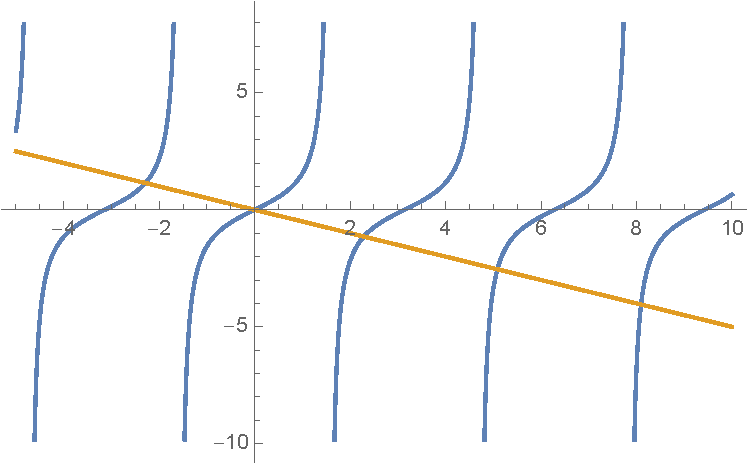
\includegraphics[width=0.6\textwidth]{2}
		\caption{}
		\label{fig:2}
	\end{figure}
%	\begin{figure}[htpb]
%		\centering
%		\begin{tikzpicture}
%			\begin{axis}[
%				xmin= -10, xmax= 20,
%				ymin= -10, ymax = 10,
%				axis lines = middle,
%			]
%				\addplot[domain=-10:20, samples=100]{-1/2*x};
%				\addplot[domain=-10:20, samples=1000]{tan(deg(x))};
%
%			\end{axis}
%
%		\end{tikzpicture}
%		\caption{}
%		\label{fig:2}
%	\end{figure}
Как видно из графиков, уравнение имеет счетное множество корней
\[\mu_1<\mu_2<\ldots,\quad \mu_k \in \left( \pi k,\,\frac{\pi}{2}+\pi k \right) , \qquad k=1,\,2,\,3,\ldots\]
Таким образом, у оператора $A$ есть счётное множество отрицательных
собственных значений и соответствующих этим собственным
значениям собственных функций
\[
	\lambda_k=- \frac{3}{\mu_k^2};\qquad u_k= \sin\left( \mu_k x \right) 
.\] 
По теореме Гильберта-Шмидта у компактного самосопряжённого
оператора существует ортогональный базис из собственных
функций в $\left( \operatorname{Ker}A \right) ^\perp$. В
нашем случае оказалось, что $\operatorname{Ker}=\{0\} $,
поэтому собственные функции
\[
u_1,\,u_2\ldots
\]
будут образовывать ортогональный базис во всём пространстве
$u \in L_2[0,\,1]$ и $\forall u \in L_2[0,\,1]$ будут
выполнены равенства
\[
	u= \sum_{k=1}^{\infty} \frac{(u,\,u_k)}{(u_k,\,u_k)}
	u_k;
\]
\[
	Au= \sum_{k=1}^{\infty} \frac{(Au,\,u_k)}{(u_k,\,u_k)}u_k
	=\sum_{k=1}^{\infty} \frac{(u,\,Au_k)}{(u_k,\,u_k)}u_k=
	\sum_{k=1}^{\infty} \lambda_k \frac{(u,\,u_k)}{(u_k,\,
	u_k)}u_k
.\] 
Итак, мы получили спектральное разложение оператора $A$.
\end{enumerate}
\item \emph{Решение уравнения}.
	\[
		u=\frac{1}{3}Au+x,\quad u \in L_2[0,\,1]
	.\] 
Выпишем разложения $u$, $Au$ и $x$ по базису $\{u_k\} $ 
\[
u=\sum_{k=1}^{\infty} \beta_k u_k,\quad
Au= \sum_{k=1}^{\infty} \lambda_k \beta_k u_k,\quad
\text{где } \beta_k=  \frac{(u,\,u_k)}{(u_k,\,u_k)};
\]
\[
x=\sum_{k=1}^{\infty} \alpha_k u_k,\quad
\text{где }\alpha_k= \frac{(x,\,u_k)}{(u_k,\,u_k)}
.\] 
Коэффициенты разложения $\alpha_k$ вычислим позднее. Подставив
все разложения в уравнение, получим
\[
\sum_{k=1}^{\infty} \beta_k u_k=\frac{1}{3} \sum_{k=1}^{\infty} \lambda_k
\beta_k u_k+ \sum_{k=1}^{\infty} \alpha_k u_k
.\] 
Приравнивая коэффициенты при каждой базисной функции, находим
\[
	\left( 1-\frac{1}{3}\lambda_k \right) \beta_k=\alpha_k,
	\quad k=0,\,1,\ldots
.\] 
\[
\beta_k= \frac{3\alpha_k}{3-\lambda_k}
.\] 
Следовательно, кандидатом на решение уравнения будет ряд
\[
u =\sum_{k=1}^{\infty} \beta_k u_k=\sum_{k=1}^{\infty}
\frac{3\alpha_k}{3-\lambda_k}u_k
.\] 
\item \emph{Проверка сходимости в $L_2[0,\,1]$}.
Поскольку
\[
\left| 1- \frac{\lambda_k}{3} \right| ^2>1,\,\quad k=1,\,2,\ldots
\] 
то справедлива оценка
\[
\sum_{k=1}^{\infty} \frac{|\alpha|^2}{|1- \lambda_k /3|^2}\| u_k\|^2\le  \sum_{k=1}^{\infty} |\alpha_k|^2\| u_k\|^2=\| x\|^2=
\int\limits_{0}^{1} x^2 dx=\frac{1}{3} 
.\] 
Значит,
\[
u= \sum_{k=1}^{\infty} \frac{3\alpha_k}{3-\lambda_k}u_k
\]
действительно является решением уравнения. Теперь осталось
только вычислить коэффициенты $\alpha_k$ 
\begin{multline*}
	\alpha_k= \frac{(x,\,u_k)}{(u_k,\,u_k)}
	=\frac{\int\limits_{0}^{1} x \sin \mu_k x \,dx}{\int\limits_{0}^{1} \sin^2 \mu_k x\, dx }=\frac{
	\left. -\frac{x}{\mu_k}\cos\mu_k x \right|_0^1+
	\frac{1}{\mu_k}\int\limits_{0}^{1} \cos\mu_k x\, dx }{
\frac{1}{2} \int\limits_{0}^{1} (1-\cos 2\mu_k x)dx }=\\=
\frac{-\frac{1}{\mu_k}\cos \mu_k +\frac{1}{\mu_k^2}\sin\mu_k}{
\frac{1}{2}-\frac{1}{4\mu_k}\sin(2\mu_k)}
.\end{multline*} 
\end{enumerate}
\end{sol}
\section{Задача Штурма-Лиувилля}
\begin{hiProb}[№11]
	Для оператора Штурма-Лиувилля $A\colon D(A)\to L_2[0,\,1]$ с областью определения
	\[
		D(A)= \left\{ f \in W^{2,\,2}\left( [0,\,1] \right) \colon f'(0)=2f(0),\ f'(1)=0 \right\} 
	\]
имеющего вид
\[
	(Af)(x)=- (x+1)^3f''(x)-3(x+1)^2f'(x),\quad
	0\le x\le 1,\ f \in D(A),
\]
найдите формулу, задающую обратный оператор $A^{-1}\colon 
L_2[0,\,1]\to D(A)$.
\end{hiProb}
\begin{sol}
Сначала преобразуем оператор $A$ к стандартному виду
\[
	(Af)(x)=-(x+1)^3 f''(x)-3(x+1)^2f'(x)=
	-\left( (x+1)^3 f'(x) \right) '
.\] 
Построим интегральное ядро оператора $A$. Решим уравнение $
(Af)(x)=0$:
\[
	-\left( (x+1)^3f'(x) \right) '=0
.\] 
\[
	(x+1)^3 f'(x)=C_1
.\] 
\[
	f'(x)=\frac{C_1}{(x+1)^3}
.\] 
\[
	f(x)= C_1 \int \frac{dx}{(x+1)^3}=-\frac{C_1}{2(x+1)^2}
	+C_2
.\] 
Найдём $f_1(x)$:
\[
	f_1'(0)=2f(0)\implies
	C_1=2C_2-C_1\implies f_1(x)=-\frac{1}{2(x+1)^2}+1
.\] 
Найдём $f_2(x)$
\[
	f'_2(1)=0 \implies \frac{C_1}{8}=0 \implies C_1=0
	\implies f_2(x)\equiv 1
.\]
Найдём определитель Вронского:
\[
	W(x)= \begin{vmatrix} - \frac{1}{2(x+1)^2}+1 & 1\\
		\frac{1}{(1+x)^3}& 0
	\end{vmatrix} 
	=-\frac{1}{(1+x)^3}
.\] 
Тогда
\[p(x)W(x)= -\frac{(x+1)^3}{(x+1)^3}=-1.\]
Выпишем интегральное ядро оператора Штурма-Лиувилля
\begin{multline*}
	G(x,\,t)=-\frac{1}{(-1)} \begin{cases}
		-\frac{1}{2(x+1)^2}+1,& 0\le x\le t\le 1,\\
		-\frac{1}{2(t+1)^2}+1,& 0\le t\le x\le 1.
	\end{cases}=\\=
	\begin{cases}
		-\frac{1}{2(x+1)^2}+1,& 0\le x\le t\le 1,\\
		-\frac{1}{2(t+1)^2}+1,& 0\le t\le x\le 1.
	\end{cases}
\end{multline*} 
Поскольку определитель Вронского $W(x)\neq 0$ для всех $x \in 
 \left[ 0,\,1 \right] $, то $\lambda=0$ не является собственным
 значением оператора $A$.
Значит, $\operatorname{Ker} A= \{0\} $ и у оператора есть
обратный оператор $A^{-1}$. Докажем, что обратный оператор
$A^{-1}$ определяется формулой
\[
	(A^{-1}g)(x)= \int\limits_{0}^{1} G(x,\,t)g(t)dt,\quad
	g \in L_2 \left[ 0,\,1 \right] ,\quad
	x \in [0,\,1]
.\] 
Для этого рассмотрим сначала произвольную функцию $g \in C[0,\,1]$ и обозначим
\[
	f(x)= \int\limits_{0}^{1} G(t,\,x)g(t)dt 
.\] 
Тогда
\[
	f(x)=\int\limits_{0}^{x} \left( -\frac{1}{2(t+1)^2}+1 \right) g(t)dt+\left( -\frac{1}{2(x+1)^2}+1 \right) \int\limits_{x}^{1}   g(t)dt
.\] 
Из свойств интегралов с переменными верхним и нижним пределами
и непрерывности функции $g$ получаем, что функция $f$ дифференцируема
на $[0,\,1]$.

Продифференцируем последнее равенство.
\begin{multline*}
	f'(x)= \frac{1}{(x+1)^3} \int\limits_{x}^{1} g(t)dt+
	\left( -\frac{1}{2(x+1)^2}+1 \right) g( x ) -
	\left( -\frac{1}{2(x+1)^2}+1 \right) g(x)=\\=
	\frac{1}{(x+1)^3} \int\limits_{x}^{1} g(t)dt 
.\end{multline*} 
Следовательно
\[
	(x+1)^3 f'(x)= \int\limits_{x}^{1} g(t)dt 
.\] 
В правой части последнего равенства подынтегральная функция
непрерывна, значит, это равенство можно продифференцировать:
\[
	\left( (x+1)^3 f'(x) \right) '=-g(x)
.\] 
Таким образом мы получили, что для любой непрерывной функции
$g(x)$ 
\[
	(Af)(x)= -\left( (x+1)^3 f'(x) \right) =g(x)
.\] 
Проверим выполнение краевых условий. Получаем:
\[
	f'(0)= \int\limits_{0}^{1} g(t)dt=2\cdot  \frac{1}{2}  \int\limits_{0}^{1} g(t)dt=2f(0)  
.\] 
\[
	f'(1)=0
.\] 
Значит
\[
	f(x)= \int\limits_{0}^{1} G(t,\,x)g(t)dt=
	(A^{-1}g)(x)
.\] 
Докажем теперь, что для всех функций $g \in L_2[0,\,1]$ обратный
оператор $(A^{-1}g)$ определяется последней формулой.

Для этого вспомним, что множество непрерывных на отрезке $[0,\,1]$
функций является всюду плотным в $L_2[0,\,1]$, поэтому для любой
функции $g \in L_2[0,\,1]$ существует последовательность
$\{g_n(x)\} $ таких, что
\begin{itemize}
	\item $\displaystyle g_n (x) \in  C[0,\,1]$ для всех $n$ ;
		\item $g_n\to g$ при $n\to \infty$ в пространстве
			$L_2[0,\,1]$.
\end{itemize}
Поскольку функции $g_n(x)$ непрерывны, то
\[
	f_n(x)= \left( A^{-1}g_n \right) (x)= \int\limits_{0}^{1} G(x,\,t)g_n(t)dt 
.\] 
Из непрерывности интегрального оператора в последнем уравнении
следует, что в пространстве $[0,\,1]$ 
\[
	f_n(x)\to f(x)= \int\limits_{0}^{1} G(x,\,t)g(t)dt 
\]
при $n\to \infty$.

Проверим теперь, что $f(x) \in D(A)$. Сначала докажем, что у
$f(x)$ есть две обобщённые производные.

Подставляя функции $f_n(x)$ и $g_n(x)$ в выражение для производной
, получаем
\[
	f_n'(x)= \frac{1}{(x+1)^3}\int\limits_{x}^{1} g_n(t)dt 
.\] 
Из непрерывности интегрального оператора следует, что в пространстве $L_2[0,\,1]$ 
\[
	f_n'(x)\to u(x)= \frac{1}{(x+1)^3} \int\limits_{x}^{1} g(t)dt 
\]
при $n\to \infty$.

Используя формулу для оператора Штурма-Лиувилля, получаем
\[
	g_n(x)=(Af_n)(x)=-(x+1)^3 f_n''(x)-3(x+1)^2f_n'(x)
.\] 
\[
	f_n''(x)=-\frac{1}{(x+1)^3}\left( g_n(x)+3(x+1)^2f_n'(x) \right) 
.\] 
\[
	f_{n}''(x)\to v(x)= -\frac{1}{(x+1)^3}\left( g(x)+
	3(x+1)^2f'(x)\right) 
.\] 
Поскольку функции $f_{n}(x) \in C^2[0,\,1]$, то их обычные
производные первого порядков являются обобщёнными производными.
Поэтому для любой финитной в $[0,\,1]$ функции $h(x)$ имеем
\[
	\int\limits_{0}^{1} f'_n(x)h(x)dx=-
	\int\limits_{0}^{1} f_n(x)h'(x)dx 
\]
и
\[
	\int\limits_{0}^{1} f''_n(x)h(x)dx= \int\limits_{0}^{1} 
	f_n h''(x)dx
.\] 
Переходя к пределу при $n\to \infty$, получаем
\[
	\int\limits_{0}^{1} u(x)h(x)= - \int\limits_{0}^{1} f(x)
	h'(x)dx
 ,\]
\[
	\int\limits_{0}^{1} v(x)h(x)dx= \int\limits_{0}^{1} f(x)
	h''(x)dx
.\] 
Таким образом, обобщённой производной $f'$ функции $f$ является
функция $u$ и справедлива формула
\[
	f'(x)=\frac{1}{(x+1)^3}\int\limits_{x}^{1} g(t)dt 
.\] 
Что и обеспечивает выполнение краевых условий.
\end{sol}
\section{Начально-краевая задача в секторе}
\begin{hiProb}[№2]
Рассмотрим сектор
\[
	G = \left\{ (x,\,y) \in \mathbb{R}^2\colon 
	x^2+y^2<\frac{1}{4},\ x>0,\ y>0\right\} 
.\] 
Пусть множество функций
\[
	D(\Delta)= \left\{ u(x,\,y) \in  C^2\left( \overline{G} \right) \colon u|_{x^2+y^2=\frac{1}{4}}=0,\ u_x|_{x=0}=0,\
	u_y|_{y=0}=0\right\} 
\]
является областью определения оператора Лапласа
\[
	\Delta\colon D(\Delta)\to L_2 \left( \overline{G} \right) 
.\] 
\begin{enumerate}
\item Доказать, что $\Delta$ --- симметричный оператор.
	\item Доказать, что $\Delta$ --- отрицательно  определён.
	\item Найти собственные значения и собственные функции
		оператора $\Delta$.
	\item Построить оператор $\overline{\Delta}$, являющийся
		замыканием оператора $\Delta$, указав его
		область определения и спектральное разложение.
	\item В $L_2 \left( \overline{G} \right) $ решить
		задачу
		\[
			\frac{d}{dt}u(t)=\overline{\Delta}u,\quad
			t>0,\ u(t) \in D(\overline{\Delta}),
		\]
		\[
			u(+0)=xy
		.\] 
\end{enumerate}
\end{hiProb}
\begin{sol}
\begin{enumerate}
\item \emph{Симметричность оператора Лапласа}. Рассмотрим
	две произвольные функции $f \in D(\Delta)$ и $g \in D(\Delta)$. Тогда
	\[
		(\Delta f,\,g)= \iint\limits_{K}^{}  \Delta
		f \cdot \overline{g}\,dx dy
	.\] 
Воспользовавшись второй формулой Грина, получаем
\[
\iint\limits_{G}^{}  \Delta f \cdot \overline{g} \, dx dy=
\oint\limits_{\partial G}^{} \left( \overline{g} \frac{\partial f}{\partial n}- f \frac{\partial \overline{g}}{\partial n} \right) dS+ \iint\limits_{G}^{}   f \Delta \overline{g} \, dx dy
,\] 
где $\partial G=\gamma_1 \cup \gamma_2 \cup \gamma_3$ и
\[
	\gamma_1= \left\{ (x,\,y)\in \mathbb{R}^2\colon 
	0\le x\le 1 /2,\ y=0\right\} 
 ,\]
\[
	\gamma_2=\left\{ (x,\,y) \in \mathbb{R}^2\colon 
	0\le y\le 1 /2,\ x=0\right\} 
 ,\]
\[
	\gamma_c= \left\{ (x,\,y) \in \mathbb{R}^2\colon 
	x^2+y^2= 1/4,\ x>0,\ y>0\right\} 
.\] 
Т.\:к.
\[
\left. \frac{\partial f}{\partial n}  \right|_{\gamma_1}=
	-f'_y|_{\gamma_1}=0;\quad \left. \frac{\partial \overline{g}}{\partial n}  \right|_{\gamma_1}=- \overline{g}'_y|_{\gamma_1}=0;
\]
\[
\left. \frac{\partial f}{\partial n}  \right|_{\gamma_2}=
	-f_x'|_{\gamma_2}=0;\quad f'_x|_{\gamma_2};\quad \left. \frac{\partial \overline{g}}{\partial n}  \right|_{\gamma_1}=0;\] 
		\[
			f_{\gamma_c}=0;\quad \overline{g}|_{\gamma_c}=0;
		\]
то
\[
	\oint\limits_{\partial G}^{} \left( \overline{g}
	\frac{\partial f}{\partial n} -f \frac{\partial \overline{g}}{\partial n}\right) dS=0 
.\] 
Следовательно,
\[
	(\Delta f,g)= \iint\limits_{G}^{} \Delta f \cdot \overline{g}\, dx dy= \iint\limits_{G}^{} f \overline{\Delta g}\,dx dy=
	(f,\,\Delta g)
.\] 
Симметричность оператора $\Delta$ доказана.
\item \emph{Отрицательная определённость оператора Лапласа}.

	Рассмотрим произвольную функцию $f \in D(\Delta)$ и воспользуемся третьей формулой Грина
\[
	(\Delta f,\,f)= \iint\limits_{G}^{}  \Delta f \cdot
	\overline{f} \, dx dy= \oint\limits_{\partial G}^{} 
	\overline{f} \frac{\partial f}{\partial n} dS-
	\iint\limits_{G}^{} |\operatorname{grad} f|^2\, dx dy 
.\] 
Поскольку $\partial G= \gamma_1 \cup \gamma_2 \cup \gamma_c$ и
\[
\left. \frac{\partial f}{\partial n}  \right|_{\gamma_1}=
	-f'_y|_{\gamma_1}=0;\quad 
	\left. \frac{\partial f}{\partial n}  \right|_{\gamma_2}=
		-f_x'|_{\gamma_2}=0;
		\quad \overline{f}|_{\gamma_c}=0
 ,\]
то
\[
\oint\limits_{\partial G}^{} \overline{f} \frac{\partial f}{\partial n} dS=0 
.\] 
Следовательно,
\[
	(\Delta f,\,f)= - \iint\limits_{G}^{} |\operatorname{grad}  f|^2\,dxdy\le 0
.\] 
Для доказательства отрицательной определённости оператора $\Delta$ остаётся проверить, что
\[
	(\Delta f,\,f)=0 \Leftrightarrow f=0
.\] 
Действительно,
\[
	(\Delta f,\,f)=0 \Leftrightarrow |\operatorname{grad} f|
	=0 \Leftrightarrow f = \operatorname{const}
.\] 
С учётом условия $f|_{\gamma_c}=0$ получаем
\[
	(\Delta f,f)=0 \Leftrightarrow f=0
.\] 
Отрицательная определённость оператора $\Delta$ доказана.
\item \emph{Собственные значения и собственные функции оператора
	Лапласа $\Delta$}

Решим краевую задачу на собственные значения для оператора 
Лапласа в секторе $G$ 
\[
\Delta f =\lambda f;\quad f|_{\gamma_c}=0,\quad
f'_y|_{\gamma_c}=0,\quad f_x'|_{\gamma_2}=0
.\] 
Для этого сначала заметим, что из симметричности и отрицательной
определённости оператора $\Delta$ следует, что собственные
значения $\lambda$ действительны и отрицательны.

Перепишем краевую задачу в полярных координатах
\[
f_{rr}+\frac{1}{r}f_r+\frac{1}{r^2}f_{\phi\phi}=\lambda f;
\quad f|_{r= 1 /2}=0,\quad
f'_\phi|_{\phi=0}=0,\quad
f'_\phi|_{\phi= \pi /2}=0
.\] 
Найдём сначала собственные функции $\Phi(\phi)$ оператора
\[
L=\frac{\partial^2}{\partial \phi^2}
\]
С областью определения
\[
	D(L)= \left\{ \Phi \in C^2 \left[ 0,\,\frac{\pi}{2} \right] \colon \Phi'(0)=0,\quad \Phi'\left( \frac{\pi}{2} \right) =0 \right\} 
.\] 
Для этого решим задачу на собственные значения
\[
	\Phi''=\mu \Phi,\quad \Phi'(0)=0,\quad \Phi'\left( 
	\frac{\pi}{2}\right) =0
.\] 
Стоит отметить, что краевые условия в данной задаче совпадают с краевыми
условиями по $\phi$ задачи в полярных координатах.

Рассмотрим три случая.
\begin{itemize}
\item $\mu>0$ 

	В этом случае общее решение уравнения в последней задаче
	имеет вид
	\[
		\Phi(\phi)= A \sh\left( \sqrt{\mu} \phi \right) +
		B \ch \left( \sqrt{\mu} \phi \right) 
	.\]
	Из краевых условий получаем
	\[
		\Phi'(0)= A\sqrt{\mu} =0;\quad
		\Phi'\left( \frac{\pi}{2} \right) =
		B \sqrt{\mu}  \sh \left( \sqrt{\mu} \frac{\pi}{2} \right) =0\implies B=0
	.\] 
Откуда следует, что у оператора $L$ нет положительных собственных
значений.
\item $\mu=0$ 

	В этом случае общее решение уравнения в последней
	задаче имеет вид
	\[
		\Phi(\phi)=A \phi+B
	.\] 
	Подставляя краевые условия последней задачи, получаем
	\[
		\Phi'(0)=A=0;\quad \Phi'\left( \frac{\pi}{2} \right) =A=0
	.\] 
	Откуда следует, что у оператора $L$ есть собственная
	функция
	\[
		\Phi_0(\phi)\equiv 1
	.\] 
	С нулевым собственным значением.
\item $\mu<0$ 

	В этом случае общее решения уравнения в последней
	задаче имеет вид
	\[
		\Phi(\phi)=A \sin \left( \sqrt{-\mu} \phi \right) +B \cos \left( \sqrt{-\mu} \phi \right) 
	.\] 
	Подставляя краевые условия последней задачи, получаем
	\[
		\Phi(0)=A \sqrt{-\mu} =0;\quad
		\Phi'\left( \frac{\pi}{2} \right) =
		-B\sqrt{-\mu} \sin \left( \sqrt{-\mu} 
		\frac{\pi}{2}\right) =0
	.\] 
	Поскольку собственная функция не может быть тождественно
	равной нулю, то
	\[
		\sin \left( \sqrt{-\mu} \frac{\pi}{2} \right) =
		0 \Leftrightarrow \sqrt{-\mu} \frac{\pi}{2}=
		\pi n \Leftrightarrow \sqrt{-\mu} =2n
	.\] 
	Таким образом, мы получили набор собственных значений
	и соответствующих им собственных функций
	\[
		\Phi_n(\phi)=\cos (2n\phi),\quad
		\mu_n=-4n^2;\quad n=1,\,2,\ldots
	.\] 
\end{itemize}
В целом все найденные собственные значения и собственные
функции можно записать одной формулой в виде
\[
	\Phi_n(\phi)=\cos (2n\phi),\quad
	\mu_n=-4n^2;\quad n=0,\,1,\,2,\ldots
\]
причём набор собственных функций $\Phi_n(\phi)$ образует
ортогональный базис в пространстве $\displaystyle L_2 \left[ 0,\,
\frac{\pi}{2}\right] $.

Теперь вернёмся к решению задачи в полярных координатах и
разложим функцию $f(r,\,\phi)$ при фиксированном $r$ в
ряд Фурье по базису $\{\cos (2n \phi)\} $ 
\[
	f(r,\,\phi)= \sum_{n=0}^{\infty} A_n(r) \cos (2n\phi)
.\] 
Подставляя это разложение в уравнение в полярных координатах,
получим
\begin{multline*}
	\sum_{n=0}^{\infty} A_n''(r) \cos (2n \phi)+
	\frac{1}{r} \sum_{n=0}^{\infty} A'_n(r) \cos (2n\phi)
	+\frac{1}{r^2} \sum_{n=0}^{\infty} (-4n^2)A_n(r)
	\cos(2n \phi)=\\= \lambda \sum_{n=0}^{\infty} A_n(r) \cos
	(2n\phi)
.\end{multline*} 
Приравнивая коэффициенты при каждом $\cos(2n\phi)$ в левой
и правой частях равенства, получаем
\[
	A''_n(r)+\frac{1}{r} A_n'(r)-\frac{4n^2}{r^2}A_n(r)=
	\lambda A_n(r),\quad n=0,\,1,\,2,\ldots
\]
Преобразуем уравнение, учитывая отрицательность $\lambda$,
к другому виду
\[
	A_n''(r)+\frac{1}{r}A'_n(r)+\left( -\lambda
	-\frac{4n^2}{r^2}\right) A_n(r)=0
.\] 
\[
	\frac{A''_n(r)}{\left( \sqrt{-\lambda}  \right) ^2}+
	\frac{1}{r \sqrt{-\lambda} }\cdot \frac{A_n'(r)}{
	\sqrt{-\lambda} }+ \left( 1-\frac{4n^2}{\left( r
\sqrt{-\lambda} \right) ^2} \right) A_n(r)=0
.\] 
Совершая в уравнении замену переменной
\[
t=r\sqrt{-\lambda} ,\] 
получаем уравнение Бесселя
\[
	A''_n(t)+\frac{1}{t}A'_n(t)+\left( 1-\frac{4n^2}{t^2} \right) A_n(t)=0
.\] 
Поскольку нас интересуют только такие решения $A_n(t)$ уравнения
Бесселя, которые ограничены в нуле, то
\[
	A_n(t)= J_{2n}(t)\implies A_n(r)=J_{2n}\left( 
	r \sqrt{-\lambda} \right) 
.\] 
Воспользовавшись краевым условием в рассматриваемом круге,
получаем
\[
	f|_{r= \frac{1}{2}}=0 \Leftrightarrow A_n (1 /2)=0
.\] 
Следовательно,
\[
	A_n(1 /2)= J_{2n} \left( \sqrt{-\lambda} /2 \right) 
 ,\] 
то есть, число $\sqrt{-\lambda} /2$ является одним из нулей
$\mu_k^{(2n)}$ функции Бесселя $J_{2n}(t)$.
Имеем выражение
\[
\sqrt{-\lambda} =2 \mu_k ^{(2n)}
.\]
Получаем набор решений уравнения
\[
	A_{n,\,k}(r)= J_{2n}\left( 2 \mu_k^{(2n)}r \right) ,\quad
	k=1,\,2,\,3,\ldots
.\] 
Итак, мы нашли собственные значения оператора Лапласа
\[
	\lambda_{n,\,k}= - \left( 2\mu_{k}^{(2n)} \right) ^2;
	\quad n=0,\,1,\,2,\ldots,\quad k=1,\,2,\,3,\ldots
\]
и соответствующие им собственные им собственные функции
\[
	f_{n,\,k}=J_{2n} \left( 2 \mu_k^{(2n)}r \right) 
	\cos (2n \phi)
.\] 
Набор собственных функций оператора Лапласа в секторе
\[
\{f_{n,\,k}\} \quad n=0,\,1,\,2,\ldots,\quad
k=1,\,2,\,3,\,\ldots
\] 
образует ортогональный базис в пространстве $L_2(K)$.
\item \emph{Спектральное разложение замыкания оператора
	Лапласа $\overline{\Delta}$}.

Мы выяснили, что оператор Лапласа $\Delta$ с областью
определения
\[
	D(\Delta)= \{f \in C^2 \left( \overline{G} \right) \colon 
	f|_{\partial G}=0\} 
\]
является симметричным и обладает в пространстве $L_2(G)$ 
ортогональным базисом из собственных функций.

Поэтому его замыкание $\overline{\Delta}$ имеет область
определения
\[
	D\left( \overline{\Delta} \right) = \{u \in L_2 (G)\colon 
	\sum_{n=0}^{\infty} \sum_{k=1}^{\infty} \lambda_{n,\,k}^2
\frac{|(u,\,f_{n,\,k})|^2}{\| f_{n,\,k}\|^2}<\infty\} 
\]
и спектральное разложение
\[
\overline{\Delta}u= \sum_{n=0}^{\infty} \sum_{k=1}^{\infty}
\lambda_{n,\,k} \frac{(u,\,f_{n,\,k})}{\| f_{n,\,k}\|^2}f_{n,\,k}
.\] 
\item \emph{Решение начально-краевой задачи}.
\[
	\frac{d}{dt}u(t)=\overline{\Delta}u(t),\quad
	t>0,\ u(t) \in D\left( \Delta \right) ,
\] 
\[
	u(+0)=xy
.\] 
\begin{enumerate}
\item Найдём \emph{<<кандидата>> на решение начально-краевой
	задачи}.

С этой целью при каждом фиксированном $t$ разложим функцию
$u(t)$ по базису $\{f_{n,\,k}\} $ 
\[
	u(t)= \sum_{n=0}^{\infty} \sum_{k=1}^{\infty}
	T_{n,\,k}(t) f_{n,\,k}
.\] 
Из спектрального разложения замыкания оператора
Лапласа $\overline{\Delta}$ получаем
\[
	\overline{\Delta} u(t)= \sum_{n=0}^{\infty}
	\sum_{k=1}^{\infty} \lambda_{n,\,k} T_{n,\,k}(t) f_{n,\,k}
.\] 
Разложим функцию $xy$ по базису $\{f_{n,\,k}\} $. Поскольку
\[
xy=\frac{1}{2} r^2 \sin 2\phi
,\] 
то её разложение по базису $\{f_{n,\,k}\} $ имеет вид
\[
xy= \sum_{n=0}^{\infty} \sum_{k=1}^{\infty} \alpha_{n,\,k} f_{n,\,k}= \sum_{n=0}^{\infty} \sum_{k=1}^{\infty} \alpha_{n,\,k}
J_{2n}\left( 2\mu_k^{(2n)}r \right) \cos(2n\phi)
.\] 
где
\begin{multline*}
	\alpha_{n,\,k}=\frac{\left( r^2 \sin 2 \phi /2,\,f_{n,\,k} \right) }{\| f_{n,\,k}\|^2}=\\=
	\frac{\iint\limits_{G}^{} \frac{1}{2}r^2 \sin 2\phi
	J_{2n}\left( 2\mu_k^{(2n)}r \right) \cos2 n \phi
r \,drd\phi}{\iint\limits_{G}^{}J_{2n}^2 \left( 2\mu_k ^{(2n)}r \right) \cos 2 n\phi r \, dr d \phi }=\\=
\frac{\int\limits_{0}^{\frac{1}{4}} \int\limits_{0}^{\frac{\pi}{2}} \frac{1}{2}r^3 \sin 2\phi J_{2n}\left( 2\mu_k ^{(2n)}r \right) 
\cos 2n \phi \,d\phi dr}{\int\limits_{0}^{\frac{1}{2}} 
\int\limits_{0}^{\frac{\pi}{2}} r J_{2n}^2 \left( 2\mu_k ^{(2n)}r \right) \cos 2n \phi \, dr d \phi}
.\end{multline*} 
Подставим найденные разложения в уравнение и начальное условие
задачи
\[
	\sum_{n=0}^{\infty}\sum_{k=1}^{\infty} T_{n,\,k}'(t)=
	\sum_{n=0}^{\infty}\sum_{k=1}^{\infty}\lambda_{n,\,k}T_{n,\,k}(t),\quad
	\sum_{n=0}^{\infty}\sum_{k=1}^{\infty}T_{n,\,k}(0)=\sum_{n=0}^{\infty}\sum_{k=1}^{\infty}\alpha_{n,\,k}
.\] 
Приравнивая коэффициенты при каждой базисной функции $f_{n,\,k}$,
для каждого $k=1,\,2,\ldots$ получаем задачу Коши
\[
	 T_{n,\,k}'(t)=
	\lambda_{n,\,k}T_{n,\,k}(t),\quad
	T_{n,\,k}(0)=\alpha_{n,\,k}
.\]
Решим эту задачу.
\[
	T_{n,\,k}(t)=C_{n,\,k} e ^{\lambda_{n,\,k}t}
.\] 
Найдём константы $C_k$ из начального условия
\[
	T_{n,\,k}(0)=C_{n,\,k} =\alpha_{n,\,k}
.\] 
Поэтому
\[
	T_{n,\,k}(t)= \alpha_{n,\,k} e^{\lambda_{n,\,k}t}
\] 
и <<кандидатом>> на решение начально-краевой задачи будет
функция
\[
	u(t)= \sum_{n=0}^{\infty} \sum_{k=1}^{\infty} 
	\alpha_{n,\,k} e^{\lambda_{n,\,k}t}f_{n,\,k}
.\] 
Проверим, что  \emph{$u(t)$ действительно является решением
задачи}. 
\item Покажем, что $\forall t>0$ $u(t) \in L_2(G)$. Оценим
	сверху квадрат нормы функции $u(t)$ используя
	равенство Парсеваля.
\begin{multline*}
	\| u(t)\|^2=\sum_{n=0}^{\infty} \sum_{k=1}^{\infty} 
	|\alpha_{n,\,k}|^2 |e^{\lambda_{n,\,k}t}|^2 \| f_{n,\,k}\|^2 =\\= \sum_{n=0}^{\infty} \sum_{k=1}^{\infty} 
	|\alpha_{n,\,k}|^2 |e^{-|\lambda_{n,\,k}|t}|^2
	\| f_{n,\,k}\|\le 
	\sum_{n=0}^{\infty} \sum_{k=1}^{\infty} 
	|\alpha_{n,\,k}|^2\| f_{n,\,k}\|^2 =
	\\= \| xy\|<\infty
.\end{multline*} 
\item Покажем, что $\forall t>0$ $u(t) \in D\left(\overline{\Delta}\right)$.
	\begin{multline*}
\| \Delta u(t)\|^2=\sum_{n=0}^{\infty} \sum_{k=1}^{\infty} 
	|\lambda_{n,\,k}|^2|\alpha_{n,\,k}|^2 |e^{\lambda_{n,\,k}t}|^2 \| f_{n,\,k}\|^2<\\<\sum_{n=0}^{\infty} \sum_{k=1}^{\infty} |\alpha_{n,\,k}|^2 \| f_{n,\,k}\|^2<\| xy\|<\infty
	\end{multline*}
	т.\:к. $\forall \lambda$ выполняется $|\lambda^2 e^{-2|\lambda|}|\le 1$.
\item  Покажем, что выполнено условие $u(+0)=xy$. Сперва покажем,
	что
\[
\sum_{n=0}^{\infty} \sum_{k=1}^{\infty} 
|\alpha_{n,\,k}|^2|e^{\lambda_{n,\,k}t}-1|^2\|f_{n,\,k}\|^2\le 
\sum_{n=0}^{\infty} \sum_{k=1}^{\infty} |\alpha_{n,\,k}|^2
\| f_{n,\,k}\|^2<\| xy\|<\infty
.\] 
Поэтому, ряд сходится, значит по признаку Вейерштрасса исходный ряд
сходится равномерно по $t$ на $(0,\,+\infty)$, следовательно
мы можем переходить к пределу по $t$ почленно, откуда следует
требуемое утверждение.
\item Докажем, что ряд $\displaystyle \sum_{n=0}^{\infty} \sum_{k=1}^{\infty} T_{n,\,k}'f_{n,\,k}$ сходится в $L_2(G)$.
\[
\sum_{n=0}^{\infty} \sum_{k=1}^{\infty} |T_{n,\,k}'|^2 \| f_{n,\,k}\|^2 = \sum_{n=0}^{\infty} \sum_{k=1}^{\infty} 
	|\lambda_{n,\,k}|^2|\alpha_{n,\,k}|^2 |e^{\lambda_{n,\,k}t}|^2 \| f_{n,\,k}\|^2<\infty
.\] 
Последнее неравенство было доказано в предыдущих пунктах
\item Докажем, что производная $u'(t)$ в $L_2(G)$ равна
	сумме ряда $\displaystyle \sum_{n=0}^{\infty} 
	\sum_{k=1}^{\infty} T_{n,\,k}'f_{n,\,k}$. В силу
	определения производной нужно доказать
	\[
		\lim_{\Delta t \to 0} \left\lVert \frac{u(t+\Delta t)-u(t)}{\Delta t}- \sum_{n=0}^{\infty} \sum_{k=1}^{\infty} 
		T'_{n,\,k}f_{n,\,k}\right\rVert^2=0
	.\] 
	Воспользуемся равенством Парсеваля и преобразуем выражение
	\begin{multline*}
	 \left\lVert \frac{u(t+\Delta t)-u(t)}{\Delta t}- \sum_{n=0}^{\infty} \sum_{k=1}^{\infty} 
		T'_{n,\,k}f_{n,\,k}\right\rVert^2=\\=
	 \left\lVert \sum_{n=1}^{\infty} \sum_{k=1}^{\infty} \frac{T_{n,\,k}(t+\Delta t)-T_{n,\,k}(t)}{\Delta t}f_{n,\,k}- \sum_{n=0}^{\infty} \sum_{k=1}^{\infty} 
		T'_{n,\,k}f_{n,\,k}\right\rVert^2=\\=
	 \sum_{n=1}^{\infty} \sum_{k=1}^{\infty} \left| \frac{T_{n,\,k}(t+\Delta t)-T_{n,\,k}(t)}{\Delta t}- 
		T'_{n,\,k}\right|^2\| f_{n,\,k}\|^2
	.\end{multline*}
По теореме Лагранжа о среднем $\forall k$ $\exists \xi_{n,\,k}
\in (t,\,t+\Delta t)$, т.ч.
$T_{n,\,k}(t+\Delta t)-T_{n,\,k}(t)=T_{n,\,k}' (\xi_{n,\,k})\Delta t$, значит
\begin{multline*}
	 \sum_{n=1}^{\infty} \sum_{k=1}^{\infty} \left| \frac{T_{n,\,k}(t+\Delta t)-T_{n,\,k}(t)}{\Delta t}- 
		T'_{n,\,k}\right|^2\| f_{n,\,k}\|^2=\\
		\sum_{n=1}^{\infty} \sum_{k=1}^{\infty} \left| T_{n,\,\,k}'(\xi_{n,\,k})- 
		T'_{n,\,k}\right|^2\| f_{n,\,k}\|^2\le \\\le 
		\sum_{n=0}^{\infty} \sum_{k=1}^{\infty} 
		\left( |T_{n,\,k}'(\xi_{n,\,k})|+
		|T_{n,\,k}'(t)|\right) ^2 \| f_{n,\,k}\|^2
.\end{multline*} 
Оценим общий член последнего ряда
\[
	|T_{n,\,k}'(t)|\le |\alpha_{n,k}|
\]
(доказано в предыдущих пунктах), значит
\[
		\left( |T_{n,\,k}'(\xi_{n,\,k})|+
		|T_{n,\,k}'(t)|\right) ^2 \| f_{n,\,k}\|^2\le 
		4|\alpha_{n,\,k}|^2\| f_{n,\,k}\|^2
.\] 
Откуда
\[
		\sum_{n=0}^{\infty} \sum_{k=1}^{\infty} 
		\left( |T_{n,\,k}'(\xi_{n,\,k})|+
		|T_{n,\,k}'(t)|\right) ^2 \| f_{n,\,k}\|^2\le 
		4\| xy\|<\infty
.\] 
Значит по признаку Вейерштрасса можем переходить к почленному
пределу по $\Delta t$, чем и доказываем требуемое утверждение.
\end{enumerate}
\end{enumerate}
\end{sol}
\end{document}
